\documentclass[11pt,a4paper]{article}
\usepackage[margin=2.4cm]{geometry}
\usepackage[T1]{fontenc}
\usepackage{lmodern}
\usepackage{amsmath,amssymb,amsthm,mathtools}
\usepackage{booktabs,graphicx,enumitem,microtype}
\usepackage{algorithm,algpseudocode}
\usepackage{xcolor}
\usepackage[colorlinks=true,linkcolor=blue!50!black,citecolor=blue!50!black,urlcolor=blue!50!black]{hyperref}
\usepackage[nameinlink,capitalise]{cleveref}

\numberwithin{equation}{section}
\newtheorem{theorem}{Theorem}[section]
\newtheorem{proposition}[theorem]{Proposition}
\newtheorem{lemma}[theorem]{Lemma}
\newtheorem{corollary}[theorem]{Corollary}
\newtheorem{conjecture}[theorem]{Conjecture}
\theoremstyle{definition}
\newtheorem{definition}[theorem]{Definition}
\newtheorem{assumption}[theorem]{Assumption}
\newtheorem{counterexample}[theorem]{Counterexample}
\newtheorem{example}[theorem]{Example}
\newtheorem{problem}[theorem]{Open problem}
\newtheorem{observation}[theorem]{Numerical observation}
\theoremstyle{remark}
\newtheorem{remark}[theorem]{Remark}

\newcommand{\R}{\mathbb{R}}
\newcommand{\T}{\mathbb{T}}
\newcommand{\Z}{\mathbb{Z}}
\newcommand{\X}{\mathcal{X}}
\newcommand{\Q}{\mathcal{Q}}
\newcommand{\Lie}{\mathcal{L}}
\newcommand{\dd}{\mathrm{d}}
\newcommand{\id}{\mathrm{id}}
\newcommand{\pf}{{}_{\#}}
\newcommand{\om}{\omega}
\newcommand{\eps}{\epsilon}
\newcommand{\abs}[1]{\lvert #1\rvert}
\newcommand{\norm}[1]{\lVert #1\rVert}
\newcommand{\status}[1]{\textnormal{\small[#1]}}
\DeclareMathOperator{\tr}{tr}
\DeclareMathOperator{\Lip}{Lip}
\DeclareMathOperator{\Diff}{Diff}
\DeclareMathOperator{\len}{len}

% Generated by prototype/make_tables.py from results/*.json -- do not edit by hand.
\newcommand{\TableHistory}{\begin{tabular}{llrrrr}\toprule
test & sampling, reconstruction & $e_\perp^{\max}$ & $e_\parallel^{\max}$ & $\oint p\,dx-c$ & $E_h-E$\\\midrule
Twist ($N=1024$, $t=40$, 39 remaps) & fixed, linear & $2.1\!\times\!10^{-3}$ & $9.8\!\times\!10^{-4}$ & $-3.3\!\times\!10^{-3}$ & $-2.1\!\times\!10^{-4}$\\
 & fixed, cubic & $2.0\!\times\!10^{-5}$ & $7.3\!\times\!10^{-6}$ & $-2.6\!\times\!10^{-5}$ & $-8.7\!\times\!10^{-7}$\\
 & fixed, AC(4,1) & $1.4\!\times\!10^{-7}$ & $7.3\!\times\!10^{-6}$ & $0$ & $-6.5\!\times\!10^{-10}$\\
 & adaptive, linear & $1.4\!\times\!10^{-2}$ & $6.3\!\times\!10^{-2}$ & $-1.4\!\times\!10^{-2}$ & $-3.7\!\times\!10^{-3}$\\
 & adaptive, AC(2,1) & $3.2\!\times\!10^{-3}$ & $4.3\!\times\!10^{-2}$ & $0$ & $-1.4\!\times\!10^{-4}$\\
 & adaptive, cubic & $7.4\!\times\!10^{-5}$ & $7.1\!\times\!10^{-4}$ & $-3.0\!\times\!10^{-5}$ & $-2.3\!\times\!10^{-6}$\\
 & adaptive, AC(4,1) & $5.2\!\times\!10^{-7}$ & $2.8\!\times\!10^{-5}$ & $0$ & $-5.8\!\times\!10^{-10}$\\
 & adaptive, quintic & $3.5\!\times\!10^{-6}$ & $1.9\!\times\!10^{-5}$ & $-2.7\!\times\!10^{-7}$ & $+1.4\!\times\!10^{-7}$\\
 & adaptive, AC(6,1) & $3.1\!\times\!10^{-8}$ & $6.4\!\times\!10^{-7}$ & $0$ & $-1.0\!\times\!10^{-9}$\\
\midrule
Collapse ($N=1024$, $t=12$, 29 remaps) & fixed, linear & $5.6\!\times\!10^{0}$ & $5.2\!\times\!10^{0}$ & $+1.1\!\times\!10^{0}$ & $-1.2\!\times\!10^{-3}$\\
 & fixed, cubic & $5.7\!\times\!10^{0}$ & $5.2\!\times\!10^{0}$ & $+1.3\!\times\!10^{0}$ & $-1.2\!\times\!10^{-3}$\\
 & fixed, AC(4,1) & $5.6\!\times\!10^{0}$ & $5.3\!\times\!10^{0}$ & $-8.3\!\times\!10^{-16}$ & $-2.1\!\times\!10^{-3}$\\
 & adaptive, linear & $7.0\!\times\!10^{-2}$ & $1.5\!\times\!10^{-1}$ & $-1.6\!\times\!10^{-4}$ & $-7.0\!\times\!10^{-4}$\\
 & adaptive, AC(2,1) & $1.3\!\times\!10^{-3}$ & $1.4\!\times\!10^{-1}$ & $+5.6\!\times\!10^{-16}$ & $+7.8\!\times\!10^{-5}$\\
 & adaptive, cubic & $1.2\!\times\!10^{-4}$ & $2.8\!\times\!10^{-3}$ & $-1.3\!\times\!10^{-5}$ & $+1.4\!\times\!10^{-7}$\\
 & adaptive, AC(4,1) & $4.3\!\times\!10^{-6}$ & $2.8\!\times\!10^{-3}$ & $-1.1\!\times\!10^{-16}$ & $+2.6\!\times\!10^{-8}$\\
 & adaptive, quintic & $5.4\!\times\!10^{-5}$ & $1.9\!\times\!10^{-3}$ & $+5.7\!\times\!10^{-6}$ & $-1.5\!\times\!10^{-9}$\\
 & adaptive, AC(6,1) & $5.0\!\times\!10^{-6}$ & $2.0\!\times\!10^{-3}$ & $0$ & $-1.5\!\times\!10^{-9}$\\
\midrule
Driven ($N=2048$, $t=12$, 29 remaps) & fixed, linear & $7.4\!\times\!10^{0}$ & $4.1\!\times\!10^{0}$ & $+1.5\!\times\!10^{1}$ & $-2.8\!\times\!10^{-3}$\\
 & fixed, cubic & $7.3\!\times\!10^{0}$ & $4.0\!\times\!10^{0}$ & $+1.7\!\times\!10^{1}$ & $-1.1\!\times\!10^{-3}$\\
 & fixed, AC(4,1) & $6.9\!\times\!10^{0}$ & $5.0\!\times\!10^{0}$ & $-5.5\!\times\!10^{-15}$ & $-7.1\!\times\!10^{-4}$\\
 & adaptive, linear & $9.0\!\times\!10^{-3}$ & $7.0\!\times\!10^{-2}$ & $-1.5\!\times\!10^{-3}$ & $-3.6\!\times\!10^{-4}$\\
 & adaptive, AC(2,1) & $9.6\!\times\!10^{-5}$ & $3.0\!\times\!10^{-2}$ & $-6.0\!\times\!10^{-16}$ & $-5.4\!\times\!10^{-5}$\\
 & adaptive, cubic & $1.3\!\times\!10^{-4}$ & $2.9\!\times\!10^{-4}$ & $+1.4\!\times\!10^{-5}$ & $+4.5\!\times\!10^{-7}$\\
 & adaptive, AC(4,1) & $2.6\!\times\!10^{-6}$ & $2.9\!\times\!10^{-4}$ & $-2.2\!\times\!10^{-16}$ & $-5.2\!\times\!10^{-8}$\\
 & adaptive, quintic & $2.2\!\times\!10^{-5}$ & $5.4\!\times\!10^{-5}$ & $-1.3\!\times\!10^{-6}$ & $+3.1\!\times\!10^{-9}$\\
 & adaptive, AC(6,1) & $4.5\!\times\!10^{-7}$ & $5.7\!\times\!10^{-5}$ & $-1.5\!\times\!10^{-15}$ & $+3.3\!\times\!10^{-9}$\\
\midrule
Comoving EdS ($N=1024$, $a\simeq 11.7$, 38 remaps) & fixed, linear & $3.8\!\times\!10^{-4}$ & $7.8\!\times\!10^{-4}$ & $-9.2\!\times\!10^{-6}$ & $-1.2\!\times\!10^{-6}$\\
 & fixed, cubic & $1.0\!\times\!10^{-7}$ & $5.1\!\times\!10^{-7}$ & $-1.2\!\times\!10^{-9}$ & $-7.3\!\times\!10^{-11}$\\
 & fixed, AC(4,1) & $5.4\!\times\!10^{-10}$ & $5.1\!\times\!10^{-7}$ & $-3.3\!\times\!10^{-16}$ & $+6.5\!\times\!10^{-10}$\\
 & adaptive, linear & $6.0\!\times\!10^{-4}$ & $1.3\!\times\!10^{-3}$ & $-2.0\!\times\!10^{-5}$ & $-6.2\!\times\!10^{-7}$\\
 & adaptive, AC(2,1) & $7.3\!\times\!10^{-7}$ & $1.5\!\times\!10^{-3}$ & $-2.8\!\times\!10^{-17}$ & $+1.2\!\times\!10^{-5}$\\
 & adaptive, cubic & $1.9\!\times\!10^{-8}$ & $7.9\!\times\!10^{-8}$ & $+1.4\!\times\!10^{-10}$ & $+8.1\!\times\!10^{-10}$\\
 & adaptive, AC(4,1) & $2.8\!\times\!10^{-11}$ & $1.1\!\times\!10^{-7}$ & $-2.2\!\times\!10^{-16}$ & $+4.5\!\times\!10^{-10}$\\
 & adaptive, quintic & $2.6\!\times\!10^{-12}$ & $1.5\!\times\!10^{-11}$ & $+1.3\!\times\!10^{-13}$ & $-1.6\!\times\!10^{-13}$\\
 & adaptive, AC(6,1) & $8.0\!\times\!10^{-14}$ & $2.2\!\times\!10^{-11}$ & $+1.7\!\times\!10^{-16}$ & $-6.0\!\times\!10^{-14}$\\
\bottomrule
\end{tabular}}
\newcommand{\TableConvergence}{\begin{tabular}{lrrrrrr}\toprule
sampling, reconstruction & $N=256$ & $N=512$ & $N=1024$ & $N=2048$ & $N=4096$ & order\\\midrule
fixed, linear & $3.2\!\times\!10^{-2}$ & $8.1\!\times\!10^{-3}$ & $2.1\!\times\!10^{-3}$ & $5.1\!\times\!10^{-4}$ & $1.3\!\times\!10^{-4}$ & 2.00\\
fixed, cubic & $4.6\!\times\!10^{-3}$ & $3.1\!\times\!10^{-4}$ & $2.0\!\times\!10^{-5}$ & $1.3\!\times\!10^{-6}$ & $8.1\!\times\!10^{-8}$ & 4.00\\
fixed, AC(4,1) & $1.2\!\times\!10^{-4}$ & $4.2\!\times\!10^{-6}$ & $1.4\!\times\!10^{-7}$ & $4.3\!\times\!10^{-9}$ & $1.4\!\times\!10^{-10}$ & 5.00\\
adaptive, linear & $1.6\!\times\!10^{-1}$ & $5.5\!\times\!10^{-2}$ & $1.4\!\times\!10^{-2}$ & $6.1\!\times\!10^{-3}$ & $1.1\!\times\!10^{-3}$ & 2.53\\
adaptive, AC(2,1) & $2.6\!\times\!10^{-2}$ & $1.4\!\times\!10^{-2}$ & $3.2\!\times\!10^{-3}$ & $5.5\!\times\!10^{-4}$ & $5.5\!\times\!10^{-5}$ & 3.31\\
adaptive, cubic & $9.8\!\times\!10^{-3}$ & $6.7\!\times\!10^{-4}$ & $7.4\!\times\!10^{-5}$ & $7.6\!\times\!10^{-6}$ & $7.5\!\times\!10^{-7}$ & 3.34\\
adaptive, AC(4,1) & $1.4\!\times\!10^{-4}$ & $9.9\!\times\!10^{-6}$ & $5.2\!\times\!10^{-7}$ & $2.4\!\times\!10^{-8}$ & $1.0\!\times\!10^{-9}$ & 4.58\\
adaptive, quintic & $1.3\!\times\!10^{-3}$ & $7.0\!\times\!10^{-5}$ & $3.5\!\times\!10^{-6}$ & $5.9\!\times\!10^{-8}$ & $1.5\!\times\!10^{-9}$ & 5.27\\
adaptive, AC(6,1) & $2.4\!\times\!10^{-5}$ & $1.4\!\times\!10^{-6}$ & $3.1\!\times\!10^{-8}$ & $5.1\!\times\!10^{-10}$ & $7.1\!\times\!10^{-10}$ & 5.92\\
\midrule
\multicolumn{7}{l}{Poincar\'e invariant error $\oint p\,dx-c$ of the carrier}\\\midrule
fixed, linear & $-5.1\!\times\!10^{-2}$ & $-1.3\!\times\!10^{-2}$ & $-3.3\!\times\!10^{-3}$ & $-8.3\!\times\!10^{-4}$ & $-2.1\!\times\!10^{-4}$ & \\
fixed, cubic & $-6.3\!\times\!10^{-3}$ & $-4.1\!\times\!10^{-4}$ & $-2.6\!\times\!10^{-5}$ & $-1.6\!\times\!10^{-6}$ & $-1.0\!\times\!10^{-7}$ & \\
fixed, AC(4,1) & $-3.6\!\times\!10^{-15}$ & $0$ & $0$ & $0$ & $0$ & \\
adaptive, linear & $-1.5\!\times\!10^{-1}$ & $-5.4\!\times\!10^{-2}$ & $-1.4\!\times\!10^{-2}$ & $-3.5\!\times\!10^{-3}$ & $-8.8\!\times\!10^{-4}$ & \\
adaptive, AC(2,1) & $-3.6\!\times\!10^{-15}$ & $+3.6\!\times\!10^{-15}$ & $0$ & $0$ & $0$ & \\
adaptive, cubic & $-6.1\!\times\!10^{-3}$ & $-3.8\!\times\!10^{-4}$ & $-3.0\!\times\!10^{-5}$ & $-2.7\!\times\!10^{-6}$ & $-2.1\!\times\!10^{-7}$ & \\
adaptive, AC(4,1) & $0$ & $0$ & $0$ & $0$ & $0$ & \\
adaptive, quintic & $+3.3\!\times\!10^{-6}$ & $+1.5\!\times\!10^{-6}$ & $-2.7\!\times\!10^{-7}$ & $-6.5\!\times\!10^{-9}$ & $-6.6\!\times\!10^{-11}$ & \\
adaptive, AC(6,1) & $0$ & $+3.6\!\times\!10^{-15}$ & $0$ & $0$ & $0$ & \\
\bottomrule\end{tabular}}
\newcommand{\TableAccumulation}{\begin{tabular}{lrrrrrrrr}\toprule
remaps in $[0,40]$ & 1 & 3 & 7 & 19 & 39 & 79 & 199 & 399\\\midrule
\multicolumn{9}{l}{$\oint p\,dx-c$}\\
adaptive, linear & $+7.8\!\times\!10^{-3}$ & $+4.6\!\times\!10^{-4}$ & $-2.1\!\times\!10^{-3}$ & $-5.9\!\times\!10^{-3}$ & $-1.4\!\times\!10^{-2}$ & $-2.4\!\times\!10^{-2}$ & $-1.9\!\times\!10^{-1}$ & $-3.7\!\times\!10^{-1}$\\
adaptive, AC(2,1) & $0$ & $0$ & $0$ & $0$ & $0$ & $0$ & $0$ & $0$\\
adaptive, cubic & $+5.4\!\times\!10^{-5}$ & $-9.0\!\times\!10^{-6}$ & $-3.0\!\times\!10^{-6}$ & $-8.0\!\times\!10^{-6}$ & $-3.0\!\times\!10^{-5}$ & $-9.5\!\times\!10^{-5}$ & $+1.1\!\times\!10^{-4}$ & $+3.8\!\times\!10^{-4}$\\
adaptive, AC(4,1) & $0$ & $0$ & $0$ & $0$ & $0$ & $0$ & $0$ & $0$\\
adaptive, quintic & $+1.7\!\times\!10^{-7}$ & $-3.8\!\times\!10^{-7}$ & $+5.7\!\times\!10^{-8}$ & $-1.1\!\times\!10^{-7}$ & $-2.7\!\times\!10^{-7}$ & $-7.7\!\times\!10^{-7}$ & $+2.3\!\times\!10^{-6}$ & $+6.7\!\times\!10^{-6}$\\
adaptive, AC(6,1) & $+3.6\!\times\!10^{-15}$ & $0$ & $0$ & $0$ & $0$ & $0$ & $0$ & $0$\\
\midrule\multicolumn{9}{l}{$e_\perp^{\max}$ at $t=40$}\\
adaptive, linear & $2.1\!\times\!10^{-3}$ & $2.3\!\times\!10^{-3}$ & $2.3\!\times\!10^{-3}$ & $9.1\!\times\!10^{-3}$ & $1.4\!\times\!10^{-2}$ & $4.1\!\times\!10^{-2}$ & $3.9\!\times\!10^{-1}$ & $2.6\!\times\!10^{0}$\\
adaptive, AC(2,1) & $5.2\!\times\!10^{-4}$ & $8.2\!\times\!10^{-5}$ & $1.2\!\times\!10^{-4}$ & $1.7\!\times\!10^{-3}$ & $3.2\!\times\!10^{-3}$ & $1.4\!\times\!10^{-2}$ & $2.6\!\times\!10^{-2}$ & $4.0\!\times\!10^{-2}$\\
adaptive, cubic & $2.2\!\times\!10^{-5}$ & $2.5\!\times\!10^{-5}$ & $2.0\!\times\!10^{-5}$ & $2.6\!\times\!10^{-5}$ & $7.4\!\times\!10^{-5}$ & $8.7\!\times\!10^{-5}$ & $2.5\!\times\!10^{-4}$ & $4.5\!\times\!10^{-4}$\\
adaptive, AC(4,1) & $5.6\!\times\!10^{-7}$ & $1.7\!\times\!10^{-7}$ & $2.9\!\times\!10^{-7}$ & $3.3\!\times\!10^{-7}$ & $5.2\!\times\!10^{-7}$ & $5.3\!\times\!10^{-7}$ & $7.3\!\times\!10^{-7}$ & $9.4\!\times\!10^{-7}$\\
adaptive, quintic & $4.0\!\times\!10^{-7}$ & $5.0\!\times\!10^{-7}$ & $3.9\!\times\!10^{-7}$ & $4.9\!\times\!10^{-7}$ & $3.5\!\times\!10^{-6}$ & $1.9\!\times\!10^{-6}$ & $2.6\!\times\!10^{-6}$ & $4.8\!\times\!10^{-6}$\\
adaptive, AC(6,1) & $6.2\!\times\!10^{-9}$ & $3.9\!\times\!10^{-9}$ & $4.2\!\times\!10^{-9}$ & $8.7\!\times\!10^{-9}$ & $3.1\!\times\!10^{-8}$ & $2.0\!\times\!10^{-8}$ & $1.2\!\times\!10^{-8}$ & $3.4\!\times\!10^{-8}$\\
\bottomrule\end{tabular}}
\newcommand{\TableComplexity}{\begin{tabular}{lrrrrr}\toprule
test & $t$ & $\mathcal A(t)$ & Euclidean length & $\max|\kappa|$ & gain $G(t)$\\\midrule
twist & 0.0 & 4.11 & 6.7 & $5.0\!\times\!10^{-1}$ & $1.8\!\times\!10^{0}$\\
 & 12.0 & 19.99 & 33.7 & $4.8\!\times\!10^{2}$ & $1.5\!\times\!10^{1}$\\
 & 24.0 & 40.43 & 69.5 & $3.8\!\times\!10^{3}$ & $1.4\!\times\!10^{1}$\\
 & 40.0 & 67.04 & 114.3 & $1.7\!\times\!10^{4}$ & $1.4\!\times\!10^{1}$\\
\midrule
spiral & 1.2 & 5.68 & 8.2 & $1.7\!\times\!10^{0}$ & $2.3\!\times\!10^{0}$\\
 & 4.8 & 15.81 & 21.8 & $5.0\!\times\!10^{4}$ & $3.1\!\times\!10^{3}$\\
 & 8.4 & 25.49 & 36.1 & $2.4\!\times\!10^{9}$ & $3.6\!\times\!10^{7}$\\
 & 12.0 & 34.60 & 50.0 & $1.4\!\times\!10^{13}$ & $8.5\!\times\!10^{10}$\\
\midrule
driven & 0.0 & 3.46 & 6.4 & $3.0\!\times\!10^{-1}$ & $1.8\!\times\!10^{0}$\\
 & 3.6 & 11.85 & 16.2 & $6.0\!\times\!10^{2}$ & $8.9\!\times\!10^{1}$\\
 & 7.2 & 24.42 & 36.6 & $2.9\!\times\!10^{7}$ & $4.9\!\times\!10^{5}$\\
 & 12.0 & 90.32 & 134.2 & $6.8\!\times\!10^{12}$ & $2.3\!\times\!10^{9}$\\
\bottomrule
\end{tabular}}
\newcommand{\TableTwoD}{\begin{tabular}{lrrrrrr}\toprule
 & \multicolumn{3}{c}{$\max|p-p^{\rm oracle}|$} & \multicolumn{3}{c}{$\max_\gamma|\oint_\gamma p\cdot dx|$}\\
reconstruction & $n=32$ & $n=64$ & $n=128$ & $n=32$ & $n=64$ & $n=128$\\\midrule
\multicolumn{7}{l}{adaptive (3 optimal-transport remaps)}\\
bilinear & $1.2\!\times\!10^{-3}$ & $4.2\!\times\!10^{-4}$ & $1.5\!\times\!10^{-4}$ & $4.2\!\times\!10^{-5}$ & $1.6\!\times\!10^{-5}$ & $8.2\!\times\!10^{-6}$\\
bicubic spline & $8.1\!\times\!10^{-6}$ & $5.3\!\times\!10^{-7}$ & $6.2\!\times\!10^{-8}$ & $3.2\!\times\!10^{-7}$ & $8.7\!\times\!10^{-9}$ & $6.2\!\times\!10^{-10}$\\
biquintic spline & $2.8\!\times\!10^{-6}$ & $1.9\!\times\!10^{-8}$ & $2.7\!\times\!10^{-10}$ & $2.0\!\times\!10^{-7}$ & $1.4\!\times\!10^{-10}$ & $1.7\!\times\!10^{-12}$\\
front-3 ($C^1$ Hermite $W$) & $9.9\!\times\!10^{-5}$ & $1.6\!\times\!10^{-5}$ & $2.9\!\times\!10^{-6}$ & $2.7\!\times\!10^{-10}$ & $1.7\!\times\!10^{-11}$ & $3.3\!\times\!10^{-11}$\\
front-5 ($C^2$ Hermite $W$) & $3.5\!\times\!10^{-5}$ & $1.1\!\times\!10^{-6}$ & $1.9\!\times\!10^{-8}$ & $1.4\!\times\!10^{-12}$ & $1.4\!\times\!10^{-13}$ & $1.4\!\times\!10^{-14}$\\
\midrule\multicolumn{7}{l}{fixed Lagrangian mesh (exact nodal data; reconstruction defect only)}\\
bilinear & -- & -- & -- & $2.4\!\times\!10^{-5}$ & $6.2\!\times\!10^{-6}$ & $1.5\!\times\!10^{-6}$\\
bicubic spline & -- & -- & -- & $8.5\!\times\!10^{-8}$ & $2.8\!\times\!10^{-9}$ & $2.0\!\times\!10^{-10}$\\
biquintic spline & -- & -- & -- & $9.7\!\times\!10^{-10}$ & $7.1\!\times\!10^{-12}$ & $8.3\!\times\!10^{-14}$\\
front-3 ($C^1$ Hermite $W$) & -- & -- & -- & $2.0\!\times\!10^{-11}$ & $2.3\!\times\!10^{-12}$ & $2.4\!\times\!10^{-12}$\\
front-5 ($C^2$ Hermite $W$) & -- & -- & -- & $2.1\!\times\!10^{-14}$ & $3.5\!\times\!10^{-15}$ & $5.8\!\times\!10^{-16}$\\
\bottomrule\end{tabular}}
\newcommand{\TableOT}{\begin{tabular}{rrrrrrr}\toprule
remap at step & $\max M/\min M$ & Newton its. & MA residual & $\lambda_{\min}(I+D^2\varphi)$ & $\int|\nabla\varphi|^2$ & point-location residual\\\midrule
30 & 1.68 & 4 & $1.5\!\times\!10^{-13}$ & 0.872 & $7.9\!\times\!10^{-5}$ & $0$\\
50 & 1.65 & 4 & $1.3\!\times\!10^{-13}$ & 0.872 & $6.4\!\times\!10^{-5}$ & $7.8\!\times\!10^{-16}$\\
70 & 1.76 & 4 & $1.1\!\times\!10^{-13}$ & 0.865 & $7.1\!\times\!10^{-5}$ & $8.9\!\times\!10^{-16}$\\
\bottomrule\end{tabular}}
\newcommand{\TableRigidity}{\begin{tabular}{llrrr}\toprule
$d$ & vertex positions & $n$ & unknowns $(p,\Sigma,c)$ & kernel dimension\\\midrule
2 & regular lattice & 5 & 77 & 15\\
2 & generic (jittered) & 5 & 77 & 3\\
2 & regular lattice & 6 & 110 & 18\\
2 & generic (jittered) & 6 & 110 & 3\\
2 & regular lattice & 8 & 194 & 24\\
2 & generic (jittered) & 8 & 194 & 3\\
3 & regular lattice & 4 & 259 & 22\\
3 & generic (jittered) & 4 & 259 & 4\\
3 & regular lattice & 5 & 503 & 28\\
3 & generic (jittered) & 5 & 503 & 4\\
\bottomrule\end{tabular}}
\newcommand{\TwoDMassErr}{$1.1\!\times\!10^{-16}$}
\newcommand{\TwoDMassRatio}{1.8}
\newcommand{\CurlRatios}{0.43, 0.22, 0.11}
\newcommand{\VNRadius}{8.9e-16}


\title{\textbf{SHAI-HULUD}\\[2pt]
\large Structure-preserving adaptive remapping of cold phase-space sheets:\\
action-augmented (Legendrian) sheets, optimal-transport sampling,\\
and the limits of discrete Lagrangian structure}
\author{CHUI project --- mathematical research note\\
\small (working manuscript; status of every statement is tracked in \cref{sec:ledger})}
\date{16 November 2026}

\begin{document}
\maketitle

\begin{abstract}
A cold collisionless medium is a Lagrangian submanifold of phase space carrying a mass measure, transported by a
Hamiltonian flow. Any discrete representation of this sheet must be re-sampled as it stretches and folds. We ask
whether Hamiltonian evolution can be coupled to an optimal-transport-guided adaptive reparameterisation without
uncontrolled violation of the physical measure and of the Hamiltonian invariants (the Lagrangian property, the
Poincar\'e--Cartan loop invariants, the Liouville class).

The continuum answer is yes for trivial reasons: reparameterisation is a gauge symmetry (relabelling), and the
Lagrangian property is the zero level of its momentum map. The discrete answer is subtler, and we establish the
following. (i)~Between remaps, a vertex method with a splitting integrator and a \emph{common-potential} force
transports an exact carrier manifold; all invariants are exactly conserved and the classical action can be
transported exactly, vertex by vertex, by the generating functions of the sub-steps (\cref{thm:action,thm:carrier}).
(ii)~All invariant violation is therefore created at remaps, with an explicit budget (\cref{thm:budget}).
(iii)~Exact element-wise preservation is impossible for piecewise-linear sheets: sliding vertices on a convex
polygon strictly loses action (\cref{cex:polygon}), and exactly isotropic P1 complexes over a lattice are rigid
(\cref{thm:rigidity}); a mass-conservative remap is not symplectic because mass and the Liouville form live in
different degrees of the de~Rham complex of the sheet (\cref{sec:derham}). (iv)~A remap is structure preserving
if and only if its normal error one-form is exact (\cref{prop:normalform}); this is achieved constructively by
reconstructing the \emph{generating function} from the transported action: in one degree of freedom by an
\emph{action-corrected interpolation} that reproduces every edge action exactly and gains one order of accuracy
in the normal direction (\cref{thm:ac}); in $d\ge 2$, chart-wise, by $C^1$ Hermite elements for the generating
function (\cref{thm:front}). (v)~Optimal transport enters only as the canonical (curl-free) choice of the label
reparameterisation that equidistributes a symplectically invariant monitor built from the cubic form of the
sheet; it never moves mass (\cref{sec:ot}).

A reference prototype with external Hamiltonians confirms the statements: in two-dimensional phase space the
action-corrected remap keeps the Poincar\'e invariant at round-off over 1--399 remaps while interpolation
remaps drift, and in chaotic and collapse tests it retains normal accuracy $10^{-6}$ where a fixed Lagrangian
mesh of the same size has $O(1)$ error; in four-dimensional phase space (single-stream regime) the
generating-function element gives circulation at quadrature round-off after Monge--Amp\`ere remaps. What is
\emph{not} established is a globally conforming exactly Lagrangian discrete carrier across caustics in $d\ge2$,
and any stability result for the self-consistent Vlasov--Poisson coupling. Individual ingredients have clear
antecedents (ColDICE, CIP schemes, wavefront construction, Monge--Amp\`ere mesh adaptation); the contribution
defended here is the structural analysis and the action-based remap, not the combination as such.
\end{abstract}

\tableofcontents

\section{Introduction and summary}\label{sec:intro}

\paragraph{Problem.} Let $\X=\T^d=\R^d/\Z^d$ be configuration space, $T^*\X=\T^d\times\R^d$ phase space with
canonical one-form $\theta=p\cdot\dd x$ and symplectic form
\begin{equation}\label{eq:omega}
\om=\dd x\wedge \dd p=-\dd\theta,\qquad \om(a,b)=a_x\cdot b_p-a_p\cdot b_x .
\end{equation}
A cold distribution is the push-forward $f_t=(F_t)\pf\mu$ of a mass measure $\mu$ on a $d$-dimensional label
manifold $\Q$ by a map $F_t:\Q\to T^*\X$, $F_t(q)=(x(q,t),p(q,t))$, which is a Lagrangian immersion. Numerical
methods that tessellate $\Q$ and move the vertices with the flow
\cite{AbelHahnKaehler2012,ShandarinHabibHeitmann2012,HahnAbelKaehler2013,HahnAngulo2016,SousbieColombi2016}
must adapt the tessellation because $F_t$ stretches without bound. The mission of this note is to decide whether
adaptation by a time-dependent reparameterisation $q=T_t(\xi)$, possibly constructed by optimal transport (OT),
can be made compatible with (a) the physical measure, (b) the Lagrangian structure, (c) selected
Poincar\'e invariants, and to derive the strongest scheme that can be defended mathematically.

\paragraph{Three distinctions that organise the paper.}
\begin{enumerate}[leftmargin=2em,itemsep=2pt]
\item \emph{Coordinate change versus projection.} A smooth reparameterisation changes nothing
(\cref{thm:gauge}). A discrete remap is a reparameterisation \emph{followed by a projection onto a
finite-dimensional family of sheets}; only the projection can violate invariants.
\item \emph{Sampling density versus mass.} OT is used on label space to choose where the degrees of freedom sit.
The mass measure is a passenger that is pulled back; no mass is transported in phase space
(\cref{prop:sampling}).
\item \emph{Conservative versus symplectic.} Mass is a top-degree form on the sheet, the Liouville form is a
closed one-form. A remap that conserves cell integrals of the former knows nothing about loop integrals of the
latter (\cref{sec:derham}).
\end{enumerate}

\paragraph{The construction in one paragraph.} Each vertex carries its label $q_i$, its phase-space position
$(x_i,p_i)$ and the \emph{action} $\Sigma_i$, a primitive of the Liouville form along the sheet,
$\dd\Sigma=F^*\theta$. The quadruple is a sample of the \emph{Legendrian lift} of the sheet to
$T^*\X\times\R$. A drift--kick integrator transports $\Sigma$ exactly. At a remap, new labels are chosen by an
OT map that equidistributes a monitor built from the measured \emph{edge action defects}
$\eps_e=\Sigma_j-\Sigma_i-\tfrac12(p_i+p_j)\cdot(x_j-x_i)$ (the symplectic area between the sheet and its chord,
a symplectic invariant that requires no finite-difference curvature estimate), and the new vertex data are read
off a reconstruction whose Liouville form is \emph{exactly} the differential of a reconstructed generating
function interpolating the $\Sigma_i$. Mass is recovered from the labels and is exact by a degree argument.

\paragraph{Conventions and standing assumptions.} Throughout, ``smooth'' means $C^\infty$ unless a finite class
is stated; $\lambda$ is Lebesgue measure on the reference torus $\Xi=\T^d$; $\Q=\T^d$ with $\mu=\rho_0\,\dd q$,
$\rho_0>0$ smooth. Maps between tori are understood through their lifts; a map ``isotopic to the identity''
lifts to $\xi\mapsto\xi+(\text{periodic})$. Results are labelled \status{established} (known; reference given),
\status{new derivation} (proved here; we do not claim that no equivalent statement exists in the literature),
\status{verified numerically}, or \status{conjecture/open}. The self-consistent Vlasov--Poisson problem for
cold data is \emph{assumed} to have a sheet solution with a $C^{1,1}$ potential on the time interval considered
(\cref{ass:regular}); this is known in $d=1$ in a weak sense \cite{ZhengMajda1994} and open in general.

\section{Continuum theory}\label{sec:continuum}

\subsection{From Hamiltonian/Vlasov dynamics to the sheet}

Let $H:T^*\X\times[0,T]\to\R$ be a (possibly time-dependent) Hamiltonian, $X_H$ its vector field,
$\iota_{X_H}\om=\dd H$, i.e.\ $\dot x=\partial_pH$, $\dot p=-\partial_xH$, and $\Phi_{t,s}$ its flow. The Vlasov
equation for a measure $f_t$ on $T^*\X$ is, in weak form,
\begin{equation}\label{eq:vlasov}
\frac{\dd}{\dd t}\int\varphi\,\dd f_t=\int\{\varphi,H_t\}\,\dd f_t\qquad\forall\varphi\in C_c^\infty(T^*\X),\qquad
\{\varphi,H\}=\dd\varphi(X_H)=\partial_x\varphi\cdot\partial_pH-\partial_p\varphi\cdot\partial_xH .
\end{equation}

\begin{definition}[cold sheet]\label{def:sheet}
A \emph{cold sheet} is a pair $(F,\mu)$ with $F:\Q\to T^*\X$ a $C^1$ immersion and $\mu=\rho_0\,\dd q$ a positive
measure on $\Q$. It represents the measure $f=F\pf\mu$. The sheet is \emph{Lagrangian} if $F^*\om=0$ and
\emph{exact with Liouville class $c\in\R^d$} if there is a function $\Sigma$ on the universal cover $\R^d$ of $\Q$ with
\begin{equation}\label{eq:exact}
\dd\Sigma=F^*\theta,\qquad \Sigma(q+e_a)=\Sigma(q)+c_a\quad(a=1,\dots,d).
\end{equation}
We call $\Sigma$ the \emph{action} (generating function) of the sheet and $(F,\Sigma):\Q\to T^*\X\times\R$ its
\emph{Legendrian lift}; the periods $c_a=\oint_{\gamma_a}p\cdot\dd x$ along the basic cycles are its Liouville class.
\end{definition}

Since $H^1(\T^d;\R)=\R^d$, every Lagrangian sheet over $\Q=\T^d$ is exact for a unique $c$, and $\Sigma$ is unique
up to a constant.

\begin{proposition}[the sheet solves Vlasov]\label{prop:vlasov}\status{established}
Let $H_t\in C^{1,1}$ in $(x,p)$ uniformly in $t$, and $F_t=\Phi_{t,0}\circ F_0$. Then $f_t=(F_t)\pf\mu$ satisfies
\eqref{eq:vlasov}. In the self-consistent case $H_t=K(p,t)+\phi_t(x)$ with $\phi_t$ determined by the density
$\rho_t=(x_t)\pf\mu$, the same holds provided $\phi_t\in C^{1,1}(\X)$.
\end{proposition}
\begin{proof}
$\frac{\dd}{\dd t}\int\varphi\,\dd f_t=\frac{\dd}{\dd t}\int_\Q\varphi(F_t(q))\,\dd\mu(q)
=\int_\Q\dd\varphi(X_{H_t})(F_t(q))\,\dd\mu(q)=\int\{\varphi,H_t\}\,\dd f_t$. The Lipschitz hypothesis gives
existence and uniqueness of the flow. In the self-consistent case the potential is a given function of $(x,t)$
once the solution is fixed, so the same computation applies.
\end{proof}

\begin{assumption}[regular sheet solution]\label{ass:regular}
For self-consistent problems we assume that a sheet solution exists on $[0,T]$ with $\phi_t\in C^{1,1}(\X)$
uniformly in $t$. For cold data this is \emph{not} a theorem in $d\ge2$ after shell crossing (densities are
singular on caustics); in $d=1$ weak measure solutions exist \cite{ZhengMajda1994}. All structural statements below
use only that each time step applies a diffeomorphism of $T^*\X$; all error estimates are proved for externally
prescribed smooth Hamiltonians.
\end{assumption}

The configuration-space density is $\rho_t=(x_t)\pf\mu$, i.e.\ $\rho_t(x)=\sum_{q:\,x(q,t)=x}\rho_0(q)/\abs{\det D_qx(q,t)}$
away from caustics $\{\det D_qx=0\}$; the number of terms is the number of streams.

\subsection{Lagrangian structure and Poincar\'e--Cartan invariants}

\begin{proposition}[invariants of the sheet]\label{prop:invariants}\status{established}
Let $F_t=\Phi_{t,0}\circ F_0$ with $H_t$ a $C^2$ function on $T^*\X$ (single valued on the torus). Then
\begin{enumerate}[label=(\roman*),leftmargin=2.2em,itemsep=1pt]
\item $F_t^*\om=F_0^*\om$; in particular a Lagrangian sheet stays Lagrangian;
\item for every closed loop $\gamma\subset\Q$ the Poincar\'e invariant $I_t[\gamma]=\oint_{F_t\circ\gamma}\theta$ is constant in time;
\item an exact sheet stays exact with the same Liouville class $c$.
\end{enumerate}
In label coordinates $F^*\om=0$ reads
\begin{equation}\label{eq:cauchy}
\partial_ax\cdot\partial_bp-\partial_bx\cdot\partial_ap=0\qquad(1\le a<b\le d).
\end{equation}
\end{proposition}
\begin{proof}
By Cartan's formula $\Lie_{X_H}\theta=\iota_{X_H}\dd\theta+\dd\iota_{X_H}\theta=\dd(\theta(X_H)-H)$, hence
\begin{equation}\label{eq:dtheta}
\frac{\dd}{\dd t}F_t^*\theta=F_t^*\Lie_{X_{H_t}}\theta=\dd\big(\mathcal{L}_t\circ F_t\big),\qquad
\mathcal{L}_t:=p\cdot\partial_pH_t-H_t .
\end{equation}
The right-hand side is exact with a single-valued primitive because $H_t$ is a function on $T^*\T^d$. Taking
$\dd$ gives (i); integrating over a closed loop gives (ii); (iii) follows from (ii) applied to the basic cycles
together with (i).
\end{proof}

\begin{remark}[Cauchy invariants and Kelvin's theorem]\label{rem:cauchy}
With $p=a^2\dot x$, \eqref{eq:cauchy} are the Cauchy invariants of Lagrangian perturbation theory
\cite{FrischVillone2014,ZheligovskyFrisch2014,RampfVilloneFrisch2015}; in a single-stream region the sheet is the
graph of the velocity field and (ii) is Kelvin's circulation theorem. The sheet formulation extends both through
shell crossing, where the Eulerian velocity is multivalued but \eqref{eq:cauchy} persists.
\end{remark}

\begin{theorem}[action transport; Legendrian lift]\label{thm:action}\status{established mathematics; new use}
\begin{enumerate}[label=(\alph*),leftmargin=2.2em,itemsep=1pt]
\item \emph{(continuous time)} If $(F_0,\Sigma_0)$ is an exact sheet, then
$\Sigma_t(q)=\Sigma_0(q)+\int_0^t\mathcal{L}_s(F_s(q))\,\dd s$ satisfies $\dd\Sigma_t=F_t^*\theta$ for all $t$, with unchanged periods.
\item \emph{(one step of a symplectic map)} Let $\Psi$ be a diffeomorphism of $T^*\X$ with
$\Psi^*\theta-\theta=\dd A_\Psi$ for a single-valued function $A_\Psi$. If $(F,\Sigma)$ is an exact sheet then so is
$(\Psi\circ F,\ \Sigma+A_\Psi\circ F)$, with the same Liouville class.
\item \emph{(splitting integrators)} For the drift $\Psi_D(x,p)=(x+D\,\nabla K(p),\,p)$ and the kick
$\Psi_\kappa(x,p)=(x,\,p-\kappa\nabla V(x))$, with $K\in C^2(\R^d)$, $V\in C^2(\X)$ and constants $D,\kappa$,
\begin{equation}\label{eq:genfun}
A_{\Psi_D}=D\,\big(p\cdot\nabla K(p)-K(p)\big),\qquad A_{\Psi_\kappa}=-\kappa\,V(x).
\end{equation}
\end{enumerate}
Consequently a kick--drift--kick scheme with arbitrary time-dependent coefficients admits an \emph{exact}
per-vertex action update: $\Sigma\mathrel{+}=D(p\cdot\nabla K-K)$ at drifts, $\Sigma\mathrel{-}=\kappa V(x)$ at kicks.
\end{theorem}
\begin{proof}
(a) is \eqref{eq:dtheta} integrated in time. (b): $(\Psi\circ F)^*\theta=F^*\Psi^*\theta=F^*\theta+\dd(A_\Psi\circ F)$.
(c): for the drift, $p\cdot\dd(x+D\nabla K(p))-p\cdot\dd x=D\,p\cdot\dd(\nabla K(p))=D\,\dd(p\cdot\nabla K-K)$; for the
kick, $(p-\kappa\nabla V)\cdot\dd x-p\cdot\dd x=-\kappa\,\dd V$. Single-valuedness of $A_{\Psi_\kappa}$ on the torus
is the periodicity of $V$.
\end{proof}

\begin{remark}
(b) is the statement that the discrete action of a symplectic map is its generating function
\cite{MarsdenWest2001,HLW}. If $V$ were not periodic (a uniform force), $A_{\Psi_\kappa}$ would be multivalued and the
Liouville class would change by $-\kappa\oint\dd V$: the periods $c_a$ record the net impulse around the box. In
periodic cosmology the mean force vanishes and $c$ is conserved.
\end{remark}

\begin{example}[initial conditions]\label{ex:ic}
Zel'dovich data $x=q+D\nabla\chi(q)$, $p=a^2\dot D\,\nabla\chi(q)$ are exactly Lagrangian with $c=0$ and
\begin{equation}\label{eq:zeldovich}
\Sigma_0=a^2\dot D\,\big(\chi+\tfrac{D}{2}\abs{\nabla\chi}^2\big),
\end{equation}
since $p\cdot\dd x=a^2\dot D\,\nabla\chi\cdot(\dd q+D\,\dd\nabla\chi)$. Second-order data
$x=q+D_1\nabla\chi_1+D_2\nabla\chi_2$, $p=a^2(\dot D_1\nabla\chi_1+\dot D_2\nabla\chi_2)$ are \emph{not}: a direct computation gives
\begin{equation}\label{eq:2lpt}
(F^*\om)_{ab}=a^2\,(D_1\dot D_2-D_2\dot D_1)\,\big[\nabla\nabla\chi_1,\nabla\nabla\chi_2\big]_{ab},
\end{equation}
the commutator of the two Hessians, a third-order quantity in the perturbation amplitude. This is the phase-space
form of the known fact that the Cauchy invariants force a transverse displacement at third order
\cite{Buchert1994,RampfVilloneFrisch2015}. Exactly Lagrangian higher-order data with a known action can be produced
by applying exact symplectic maps (e.g.\ kick--drift steps with perturbative potentials) to Zel'dovich data and
using \cref{thm:action}(b).
\end{example}

\subsection{Reparameterisation as a gauge symmetry}

\begin{theorem}[relabelling invariance]\label{thm:gauge}\status{new derivation; elementary}
Let $(F,\Sigma,\mu)$ be an exact cold sheet and $T:\Xi\to\Q$ a $C^1$ diffeomorphism isotopic to the identity. Put
$G=F\circ T$, $\tilde\Sigma=\Sigma\circ T$, $\tilde\mu=T^*\mu:=(T^{-1})\pf\mu$, i.e.\ $\tilde\rho=(\rho_0\circ T)\det DT$. Then
\begin{enumerate}[label=(\roman*),leftmargin=2.2em,itemsep=1pt]
\item $G\pf\tilde\mu=F\pf\mu$ (the physical distribution is unchanged);
\item $G^*\om=T^*(F^*\om)=0$ and $\dd\tilde\Sigma=G^*\theta$ with the same periods $c$;
\item if $F_t$ solves Hamilton's equations and $T_t$ is any $C^1$ family of such diffeomorphisms, then
$G_t=F_t\circ T_t$, $q_t=T_t$, $\tilde\Sigma_t=\Sigma_t\circ T_t$, $\tilde\rho_t$ satisfy the arbitrary
Lagrangian--Eulerian system on $\Xi$
\begin{equation}\label{eq:ale}
\begin{aligned}
\partial_tG&=X_{H_t}(G)+(w\cdot\nabla_\xi)G,&\qquad \partial_tq&=(w\cdot\nabla_\xi)q,\\
\partial_t\tilde\Sigma&=\mathcal{L}_t(G)+(w\cdot\nabla_\xi)\tilde\Sigma,&\qquad \partial_t\tilde\rho&=\nabla_\xi\cdot(\tilde\rho\,w),
\end{aligned}
\end{equation}
with mesh velocity $w=(DT_t)^{-1}\partial_tT_t$, and conversely.
\end{enumerate}
The conclusions (i)--(ii) fail if $T$ is not injective (mass is counted with multiplicity) or does not preserve
the homology classes of the basic cycles (the periods are permuted).
\end{theorem}
\begin{proof}
(i) $G\pf T^{-1}\pf\mu=(F\circ T\circ T^{-1})\pf\mu$. (ii) Pull-back commutes with $\dd$; a map isotopic to the
identity acts trivially on $H_1$. (iii) Differentiate $G_t(\xi)=F_t(T_t(\xi))$:
$\partial_tG=X_H(G)+D_qF\,\partial_tT=X_H(G)+D_\xi G\,(DT)^{-1}\partial_tT$; the other equations are the same
computation, and the last is the continuity equation for the push-forward by $T_t^{-1}$, whose velocity is $-w$.
\end{proof}

Equation \eqref{eq:ale} shows what a remap \emph{is}: an advection in the reference coordinates of the four
fields $(G,q,\tilde\Sigma,\tilde\rho)$ by the mesh velocity. The advection is where a discretisation can damage
structure; the Hamiltonian part cannot (\cref{thm:carrier}).

\begin{theorem}[the Lagrangian condition is a momentum map]\label{thm:momentum}\status{established \cite{Donaldson1999}}
On the space $\mathcal M$ of maps $F:\Q\to T^*\X$ consider the symplectic form
$\Omega_F(\delta_1F,\delta_2F)=\int_\Q\om(\delta_1F,\delta_2F)\,\dd\mu$. The group $\Diff_\mu(\Q)$ of
$\mu$-preserving diffeomorphisms acts by $F\mapsto F\circ\eta^{-1}$, preserving $\Omega$ and every Hamiltonian of
the form $\mathcal H(F)=\int_\Q H\circ F\,\dd\mu+\tfrac12\iint\mathcal G(x(q)-x(q'))\,\dd\mu\,\dd\mu$. For a
$\mu$-divergence-free vector field $v$ on $\Q$ the function
\begin{equation}\label{eq:momentum}
J_v(F)=\int_\Q (F^*\theta)(v)\,\dd\mu
\end{equation}
generates the infinitesimal action $F\mapsto DF\cdot v$: $\dd J_v=\iota_{DF\cdot v}\Omega$. Hence $J_v$ is conserved by
the dynamics for every such $v$, and $J_v(F)=0$ for all $\mu$-divergence-free $v$ with zero mean flux if and only
if $F^*\theta$ is closed, i.e.\ $F$ is Lagrangian; the values on the harmonic (constant-flux) fields are the periods
$c_a$.
\end{theorem}
\begin{proof}
For a variation $Y$ of $F$ (a vector field along $F$), $\delta(F^*\theta)=F^*(\iota_Y\dd\theta)+\dd(\theta(Y))$, so
$\delta J_v=\int_\Q\dd\theta(Y,DF\,v)\,\dd\mu+\int_\Q\Lie_v(\theta(Y))\,\dd\mu
=\int_\Q\om(DF\,v,Y)\,\dd\mu$, the last integral vanishing because $\Lie_v\mu=0$. The characterisation of the zero
level is the Hodge--Helmholtz statement that the annihilator of the $\mu$-divergence-free fields is the space of exact one-forms.
\end{proof}

\begin{remark}[what a discretisation loses]\label{rem:noether}
\Cref{thm:momentum} is the Noether explanation of \cref{prop:invariants}: the Lagrangian property is conserved
\emph{because} the cold sheet has the relabelling symmetry of a fluid \cite{Salmon1988}. A vertex discretisation
$\mathcal M_h=(T^*\X)^N$ retains at most the permutation subgroup, so no discrete Noether theorem can deliver exact
Lagrangian structure of an interpolant. Exactness must come from a different mechanism (\cref{thm:carrier}).
The full relabelling group $\Diff(\Q)$ fibres over the space of densities with fibre $\Diff_\mu$; the
structure-relevant information of a reparameterisation is entirely in the base (the sampling density), which is
why optimal transport, the horizontal lift of this fibration \cite{Otto2001}, is the natural selector (\cref{sec:ot}).
\end{remark}

\subsection{Which perturbations of a sheet preserve the structure?}

A remap replaces the sheet by a nearby one. The following elementary statement identifies exactly which
perturbations are harmless.

\begin{proposition}[normal form of structure-preserving perturbations]\label{prop:normalform}\status{new derivation; the nonlinear version is \cite{Weinstein1971}}
Let $(F,\Sigma)$ be an exact Lagrangian immersion and $F^\varepsilon=F+\varepsilon e+O(\varepsilon^2)$ a smooth family
of immersions. Define the \emph{normal error one-form} $\beta_e\in\Omega^1(\Q)$,
\begin{equation}\label{eq:beta}
\beta_e(v):=\om(e,DF\,v)=e_x\cdot\partial_vp-e_p\cdot\partial_vx .
\end{equation}
Then
\begin{equation}\label{eq:varliouville}
\frac{\dd}{\dd\varepsilon}\Big|_{0}(F^\varepsilon)^*\theta=-\beta_e+\dd\big(\theta(e)\big),\qquad
\frac{\dd}{\dd\varepsilon}\Big|_{0}(F^\varepsilon)^*\om=\dd\beta_e .
\end{equation}
Consequently: (i) $\beta_e$ vanishes for tangential perturbations $e=DF\,v$ (relabelling) and
$e_\perp\mapsto\beta_e$ is an isomorphism from normal fields to one-forms; (ii) to first order the perturbed sheet is
Lagrangian iff $\dd\beta_e=0$, and it keeps the Liouville class iff $\beta_e$ is exact, $\beta_e=\dd\sigma$, in which case
its action is $\Sigma+\varepsilon(\theta(e)-\sigma)$; (iii) of the $d$ independent normal components of a generic
error field, structure preservation leaves exactly one scalar function $\sigma$ free. In $d=1$ every $\beta_e$ is
closed and the only obstruction is the single number $\oint_\Q\beta_e$ (the change of enclosed action).
\end{proposition}
\begin{proof}
For a family of maps with variation field $e$, $\frac{\dd}{\dd\varepsilon}F_\varepsilon^*\theta=F^*(\iota_e\dd\theta)+\dd(F^*\iota_e\theta)$
and $(\iota_e\dd\theta)(DF\,v)=-\om(e,DF\,v)$. Tangential fields give zero because $F$ is Lagrangian. Since $DF(T_q\Q)$
is a Lagrangian subspace, $\om$ identifies the quotient $T(T^*\X)/DF(T\Q)$ with $T^*\Q$, which is (i). (ii) and (iii)
are read off \eqref{eq:varliouville}.
\end{proof}

The nonlinear version is Weinstein's theorem: a neighbourhood of an embedded Lagrangian $\Lambda$ is
symplectomorphic to a neighbourhood of the zero section of $T^*\Lambda$, nearby Lagrangians are graphs of closed
one-forms, and those with the same Liouville class are graphs of $\dd\sigma$. Equivalently they are the images of
$\Lambda$ under Hamiltonian diffeomorphisms: an exact remap is indistinguishable from a small symplectic kick.
In the same spirit, every tangential (sliding) vector field on $\Lambda$ is the restriction of the Hamiltonian
vector field of a function vanishing on $\Lambda$, because $X_K$ is tangent to a Lagrangian $\Lambda$ iff
$\dd K|_{T\Lambda}=0$; reparameterisation is therefore not merely compatible with, but internal to, the symplectic category.

\begin{proposition}[cubic form]\label{prop:cubic}\status{new derivation; classical object in affine/Lagrangian geometry}
For a Lagrangian immersion $F$ define
\begin{equation}\label{eq:cubic}
C_{abc}:=\om(\partial_aF,\partial_b\partial_cF)=\partial_ax\cdot\partial_{bc}p-\partial_ap\cdot\partial_{bc}x .
\end{equation}
Then $C$ is a totally symmetric $(0,3)$ tensor field on $\Q$ (it transforms tensorially under relabelling), and it
is invariant under affine symplectic maps of phase space. For a graph $p=\nabla\phi(x)$ parameterised by $x$,
$C=D^3\phi$. In $d=1$, $C=\kappa\,\dd q^3$ with $\kappa=\om(F',F'')$, and $\abs{\kappa}^{1/3}\dd q$ is the
equi-affine arclength element of the curve.
\end{proposition}
\begin{proof}
Differentiating $\om(\partial_aF,\partial_cF)=0$ with respect to $q^b$ gives
$\om(\partial_{ab}F,\partial_cF)+\om(\partial_aF,\partial_{bc}F)=0$, i.e.\ $C_{abc}=C_{cab}$; with the obvious symmetry in
$(b,c)$ this is total symmetry. Under a change of labels the second derivatives acquire terms
$\Gamma^e_{bc}\partial_eF$, which are annihilated by $\om(\partial_aF,\cdot)$. An affine symplectic map commutes with
differentiation and preserves $\om$. The graph case is immediate.
\end{proof}

The cubic form is the lowest-order symplectic invariant of the \emph{shape} of the sheet; it will control both the
Lagrangian defect of piecewise-linear interpolation (\cref{prop:flux}) and the natural monitor function (\cref{sec:monitor}).

\section{Optimal transport of the sampling}\label{sec:ot}

\subsection{Equidistribution and its indeterminacy}

Fix a reference torus $\Xi=\T^d$ carrying a fixed mesh (uniform, or a fixed hierarchy). A discrete sheet is
parameterised over $\Xi$ through a \emph{label map} $T:\Xi\to\Q$. Let $M:\Q\to(0,\infty)$ be a \emph{monitor
density}, $\int_\Q M\,\dd q=1$, expressing where resolution is wanted (\cref{sec:monitor}). The
\emph{equidistribution principle} asks that reference cells of equal volume carry equal monitor mass:
\begin{equation}\label{eq:equi}
T\pf\lambda=\nu_M:=M\,\dd q\qquad\Longleftrightarrow\qquad M(T(\xi))\,\det DT(\xi)=1 .
\end{equation}
For $d\ge2$ this is one scalar equation for $d$ unknown functions: if $T$ solves \eqref{eq:equi} so does
$s\circ T$ for every $\nu_M$-preserving diffeomorphism $s$. The indeterminacy is exactly the fibre $\Diff_{\nu_M}$
of \cref{rem:noether}; its elements shear and rotate cells without changing their monitor mass, and they are
harmful (they degrade mesh quality and enlarge the constants of every interpolation estimate) but invisible to \eqref{eq:equi}.

\subsection{The transport problem and its well-posedness}

\begin{definition}[sampling transport problem]\label{def:ot}
Given $M$, find
\begin{equation}\label{eq:monge}
T=\arg\min\Big\{\int_\Xi d_{\T^d}(\xi,T(\xi))^2\,\dd\xi\ :\ T\pf\lambda=\nu_M\Big\},
\end{equation}
where $d_{\T^d}$ is the flat distance on the torus (we identify $\Xi$ and $\Q$ as flat tori).
\end{definition}

\begin{theorem}[existence, uniqueness, structure, regularity]\label{thm:ot}\status{established
\cite{Brenier1991,Cordero1999,McCann2001,Caffarelli1992}}
Let $M\in C^{k,\alpha}(\Q)$, $k\ge0$, $0<\alpha<1$, with $0<m_-\le M\le m_+$. Then \eqref{eq:monge} has a unique
minimiser. It has the form
\begin{equation}\label{eq:brenier}
T(\xi)=\xi+\nabla\varphi(\xi)\pmod{\Z^d},\qquad \varphi\ \text{periodic},\qquad \tfrac12\abs{\xi}^2+\varphi\ \text{convex},
\end{equation}
$\varphi\in C^{k+2,\alpha}$ solves the Monge--Amp\`ere equation
\begin{equation}\label{eq:ma}
M\big(\xi+\nabla\varphi(\xi)\big)\,\det\big(I+D^2\varphi(\xi)\big)=1 ,
\end{equation}
and $T$ is a $C^{k+1,\alpha}$ diffeomorphism isotopic to the identity. Conversely a periodic $\varphi$ with
$I+D^2\varphi>0$ solving \eqref{eq:ma} gives the minimiser.
\end{theorem}

The selection made by \eqref{eq:monge} has three properties that matter here. \emph{(a) Canonical gauge.} Among all
equidistributing maps the optimal one is the unique gradient map (Brenier's polar factorisation: every
equidistributing map is $T\circ s$ with $s$ measure preserving); its displacement is curl free, which removes the
harmful fibre directions. \emph{(b) No tangling.} $I+D^2\varphi>0$ makes $T$ a diffeomorphism; in computations the
smallest eigenvalue of $I+D^2\varphi$ is a certificate. \emph{(c) Memorylessness.} $T$ depends only on the current
monitor, not on the history of the mesh; composing increments would not have this property (a composition of
gradient maps is not a gradient map) and would accumulate shear. Optimal-transport mesh adaptation with these
properties is well established for PDE meshes in physical space
\cite{BuddWilliams2006,BuddHuangRussell2009,Delzanno2008,Weller2016}; the present use differs only in \emph{where}
it acts (label space of a Lagrangian sheet) and in what it is allowed to touch (\cref{prop:sampling}).

\begin{proposition}[$d=1$: monotone rearrangement]\label{prop:ot1d}\status{established}
For $d=1$ the equidistributing orientation-preserving maps of the circle form a one-parameter family
$T_\tau=C^{-1}(\cdot+\tau)$, $C(q)=\int_{0}^{q}M$, and \eqref{eq:monge} selects the offset $\tau$ by a
one-dimensional minimisation \cite{DelonSalomonSobolevski2010}. Optimal transport therefore adds nothing to
equidistribution in $d=1$ beyond fixing a rotation; the prototype pins the label $q=0$ instead.
\end{proposition}

\paragraph{Linearisation and solution.} With $F(\varphi)=\log\det(I+D^2\varphi)+\log M(\xi+\nabla\varphi)$,
\begin{equation}\label{eq:malin}
F'(\varphi)[\psi]=\tr\big((I+D^2\varphi)^{-1}D^2\psi\big)+\nabla\log M(T)\cdot\nabla\psi ,
\end{equation}
a uniformly elliptic operator on admissible $\varphi$, equal to the Laplacian at $\varphi=0$, $M=1$; for
$M=1+\varepsilon m$ one has $\Delta\varphi=-\varepsilon m+O(\varepsilon^2)$. The prototype solves \eqref{eq:ma} by a
damped Newton iteration with \eqref{eq:malin} inverted by GMRES preconditioned with the FFT inverse Laplacian and
a backtracking line search that maintains $I+D^2\varphi>0$ (\texttt{solve\_ot} in \texttt{prototype/sheet2d.py}).
Measured behaviour is reported in \cref{sec:num2d}.

\subsection{Sampling is not mass}

\begin{proposition}[the physical measure is a passenger]\label{prop:sampling}\status{new derivation; elementary}
Let $T_0,T_1:\Xi\to\Q$ be two label maps and $F$ a sheet with mass measure $\mu$.
\begin{enumerate}[label=(\roman*),leftmargin=2.2em,itemsep=1pt]
\item If the reference density is updated as a pull-back, $\tilde\mu_i=T_i^*\mu$, both discretisations represent the
same measure $F\pf\mu$, for arbitrary monitors. The reference density is $\tilde\rho=(\rho_0\circ T)\det DT=(\rho_0/M)\circ T$:
cell masses necessarily vary by the factor $\max(M/\rho_0)/\min(M/\rho_0)$.
\item If instead the masses stay attached to the moved sample points (the reference density is kept,
$\tilde\mu_1:=\tilde\mu_0$), the represented measure becomes $F\pf(R\pf\mu)$ with $R=T_1\circ T_0^{-1}$, and
\begin{equation}\label{eq:w2}
W_2\big(F\pf R\pf\mu,\,F\pf\mu\big)\le\Lip(F)\,\norm{R-\id}_{L^2(\mu)},
\end{equation}
with equality to leading order for small displacements along a single stream. This is an $O(1)$ modification of the
distribution function unless $R\pf\mu=\mu$.
\item Equal-mass sampling and adaptive sampling are incompatible: $\tilde\rho$ constant forces $T\pf\lambda\propto\mu$,
leaving only the gauge freedom $\Diff_\mu$.
\end{enumerate}
\end{proposition}
\begin{proof}
(i) is \cref{thm:gauge}(i). (ii) $(F\circ T_1)\pf(T_0^{-1})\pf\mu=F\pf R\pf\mu$; the coupling $(F\circ R,F)\pf\mu$ gives
the bound. (iii) is \eqref{eq:equi} with $M=\rho_0/\mu(\Q)$.
\end{proof}

This is the precise sense in which the optimal transport of \cref{def:ot} must be distinguished from the uses of
optimal transport that \emph{do} move mass in cosmology: Monge--Amp\`ere--Kantorovich reconstruction and its
semi-discrete descendants \cite{FrischEtAl2002,BrenierEtAl2003,LevyEtAl2021} transport the mass density in
\emph{configuration space} between initial and final times and are restricted to single-stream (convex-potential)
maps. Here the transported measure is Lebesgue measure on a reference torus, the target is a sampling density on
label space, and the phase-space measure is invariant by construction, in any number of streams.

\subsection{A symplectically invariant monitor}\label{sec:monitor}

What should be equidistributed? Phase space has no canonical metric ($x$ and $p$ have different units), so
curvature-based monitors depend on an arbitrary scaling. The action supplies an invariant alternative.

\begin{lemma}[edge action defect]\label{lem:edge}\status{new derivation; verified symbolically}
Let $(F,\Sigma)$ be an exact $C^4$ sheet, $q_0\in\Q$, $e\in\R^d$ a label-space edge vector of length $h$, and
$z_0=F(q_0)$, $z_1=F(q_0+e)$. The \emph{edge action defect}
\begin{equation}\label{eq:edgedefect}
\eps_e:=\Sigma(q_0+e)-\Sigma(q_0)-\tfrac12(p_0+p_1)\cdot(x_1-x_0)
\end{equation}
is the signed symplectic area between the sheet arc over the edge and its chord, and
\begin{equation}\label{eq:edgeexp}
\eps_e=-\tfrac1{12}\,C(e,e,e)+O(h^4),
\end{equation}
with $C$ the cubic form \eqref{eq:cubic} at $q_0$.
\end{lemma}
\begin{proof}
$\Sigma(q_0+e)-\Sigma(q_0)=\int_0^1p\cdot\partial_sx\,\dd s$ along $s\mapsto F(q_0+se)$, and the trapezoid term is the
integral of $\theta$ along the chord, so $\eps_e=\oint\theta$ over the closed curve arc--minus--chord, which is the
signed area by Stokes. Expanding $x,p$ to third order in $s$,
$\tfrac12(p_0+p_1)\cdot(x_1-x_0)-\int_0^1p\cdot x'\,\dd s=\tfrac1{12}(x'\cdot p''-p'\cdot x'')+O(h^4)$ with
derivatives along $e$ at $s=0$, which is $\tfrac1{12}\om(\partial_eF,\partial_e^2F)$.
\end{proof}

$\eps_e$ is computable from vertex data alone, exactly (no finite differences), and is invariant under affine
symplectic maps of phase space (it is an area); it is the local quantity a piecewise-linear
representation gets wrong. Requiring $\abs{\eps_e}$ to be equidistributed for edges of local length $h(q)$, with
node density $h^{-d}$ and $N$ nodes, the standard variational argument (minimise $\int\norm{C}h^{3-d}\dd q$ subject
to $\int h^{-d}\dd q=N$) gives
\begin{equation}\label{eq:monitor}
M\ \propto\ \norm{C}^{\,d/(3+d)}\quad(L^1\text{-optimal}),\qquad M\ \propto\ \norm{C}^{\,d/3}\quad(\text{max-optimal}).
\end{equation}

\paragraph{The case $d=1$: equi-affine sampling and a complexity functional.} Here $C=\kappa\,\dd q^3$ and the
max-optimal monitor is $M\propto\abs{\kappa}^{1/3}$, i.e.\ \emph{uniform sampling in equi-affine arclength}, the
arclength that is invariant under area-preserving affine maps of the phase plane. This connects to the classical
theory of best polygonal approximation of convex curves in the area metric \cite{McClureVitale1975}. Writing
\begin{equation}\label{eq:complexity}
\begin{gathered}
\mathcal A(t):=\int_\Q\abs{\kappa(q,t)}^{1/3}\dd q,\qquad
\eps_{\rm equi}=\frac{\mathcal A^3}{12N^3},\qquad
\eps_{\rm unif}=\frac{\abs{\Q}^3\max\abs\kappa}{12N^3},\\
G(t):=\frac{\eps_{\rm unif}}{\eps_{\rm equi}}=\frac{\abs{\Q}^3\max_q\abs\kappa}{\mathcal A(t)^3}\ \ge1 ,
\end{gathered}
\end{equation}
$\mathcal A$ is a symplectic invariant measuring the intrinsic cost of representing the sheet by chords, and $G$ is
the gain of adaptive over fixed (uniform-in-label) sampling at equal $N$ ($G\ge1$ by H\"older). Adaptivity cannot
reduce $\mathcal A$; it can only remove $G$. The measured growth of $\mathcal A$ and $G$ is reported in
\cref{tab:complexity}: in the collapse and chaotic tests $\mathcal A$ grows roughly linearly while $G$ grows
exponentially.

\begin{remark}[regularisation and regularity of the monitor]\label{rem:monreg}
\eqref{eq:monitor} degenerates where $C=0$ and ignores higher-order error terms; practical monitors add a floor and
arclength/turning-angle terms (prototype: \texttt{monitor\_density}). More importantly, \emph{the remap error
inherits the regularity of $T$}: an interpolation estimate of order $r$ in the reference coordinates involves
$\norm{F\circ T}_{W^{r,\infty}}$, hence $r$ derivatives of $T$, hence $r-1$ derivatives of $M$ by \cref{thm:ot}. In
the $d=2$ prototype a monitor with a kink ($\norm{C}$ at a zero of $C$) smoothed only at the mesh scale reduced
the observed remap order to about one; a monitor mollified at a fixed label-space scale restored the design
order (\cref{sec:num2d}). In $d=1$ the prototype interpolates directly on the non-uniform label nodes, so the
regularity of $T$ does not enter. Finally, optimal transport controls a scalar density only: it cannot align cells
with the anisotropy of the tensor $C$; anisotropic (metric-based) refinement as in ColDICE addresses a complementary need.
\end{remark}

\section{Discrete geometry of sheets}\label{sec:discrete}

\subsection{Discrete sheets, carriers, and the discrete Liouville cochain}

\begin{definition}[discrete Legendrian sheet]\label{def:discrete}
Let $\mathcal K$ be a mesh of the reference torus $\Xi$ (simplicial or tensor-product) with node set $\{\xi_i\}$.
A \emph{discrete Legendrian sheet} is the nodal data
\begin{equation}\label{eq:state}
Z=\{(q_i,\ x_i,\ p_i,\ \Sigma_i)\}_i\ \subset\ \Q\times T^*\X\times\R ,
\end{equation}
understood on the universal cover ($q$, $x$ and $\Sigma$ are quasi-periodic with periods $e_a$, $e_a$, $c_a$).
A \emph{reconstruction} is an operator $\mathcal R:Z\mapsto(G_h,q_h)$ producing continuous piecewise-$C^1$ maps on
$\Xi$ interpolating the nodal values. A \emph{carrier} of $Z$ is any continuous piecewise-$C^1$ extended sheet
$(G,q,\Sigma):\Xi\to T^*\X\times\Q\times\R$ through the nodal data; it is an \emph{exact Lagrangian carrier} if
$\dd\Sigma=G^*\theta$. The \emph{discrete Liouville cochain} of a reconstruction assigns to each mesh edge $e$ the
number $\alpha_h(e)=\int_eG_h^*\theta$; the reconstruction is \emph{action consistent} if
$\alpha_h(e)=\Sigma_j-\Sigma_i$ on every edge $e=(i,j)$.
\end{definition}

A finite point set lies on infinitely many Lagrangian manifolds, so ``the vertices lie on a Lagrangian manifold''
has no content by itself. The notion of carrier becomes meaningful through \cref{thm:carrier}: the scheme
\emph{determines} a specific carrier at all times, and statements about invariants are statements about it.
Action consistency is a closedness statement: if $\alpha_h=\delta\Sigma$ then the flux of $G_h^*\om$ through every
mesh 2-cell vanishes and every mesh-loop integral of $\theta$ takes its exact value.

\subsection{Piecewise-linear and quadratic elements}

\begin{proposition}[Lagrangian defect of P1 interpolation]\label{prop:flux}\status{new derivation; verified symbolically}
Let $F$ be a $C^4$ Lagrangian immersion and $G_h$ its piecewise-linear interpolant on a label-space triangle
$\tau$ with vertices $q_0,q_0+u,q_0+v$, $\abs u,\abs v\le h$. Then
\begin{equation}\label{eq:flux}
\int_\tau G_h^*\om=-\oint_{\partial\tau}G_h^*\theta=-\tfrac14\big[C(u,u,v)-C(u,v,v)\big]+O(h^4).
\end{equation}
Thus the P1 interpolant of a Lagrangian sheet is not Lagrangian; its defect per unit label area is $O(h)$ and is
governed by the cubic form.
\end{proposition}
\begin{proof}
On each straight edge $\int\theta$ is the trapezoid value, which by \cref{lem:edge} exceeds the exact edge action by
$\tfrac1{12}C(e,e,e)+O(h^4)$. The exact actions sum to zero around $\partial\tau$ because $F^*\theta$ is closed, and
$\tfrac1{12}[u^3+(v-u)^3+(-v)^3]=\tfrac14[u^2v-uv^2]$ in the symmetric algebra, the base-point dependence of $C$
contributing $O(h^4)$.
\end{proof}

For the graph of $\phi=x_1^2x_2$ on the triangle $(0,0),(h,0),(0,h)$, \eqref{eq:flux} is exact:
$\oint\theta_{PL}=h^3/2$. For quadratic elements with a mid-edge tracer at the parametric midpoint, the edge
action is given by a Simpson-type formula and its error is $O(h^5)$ (measured orders $4.93,\,4.98,\,5.00$), so the
flux defect per unit area is $O(h^3)$: smaller, still not zero.

\subsection{Mass}\label{sec:mass}

\begin{proposition}[total mass is a degree]\label{prop:mass}\status{new derivation; elementary}
Let $q_h:\Xi\to\Q$ be continuous, piecewise $C^1$ and homotopic to the identity, and define cell masses
$m_K=\int_K q_h^*\mu=\int_K\rho_0(q_h)\det Dq_h\,\dd\xi$. Then $\sum_Km_K=\mu(\Q)$ exactly, for \emph{every} such
$q_h$; all $m_K$ are positive iff $q_h$ is orientation preserving on every cell. For P1 labels and uniform $\mu$,
$m_K$ is the signed volume of the label simplex.
\end{proposition}
\begin{proof}
$\int_\Xi q_h^*\mu=\deg(q_h)\int_\Q\mu$ and the degree of a map homotopic to the identity is one.
\end{proof}

Hence the total mass is conserved by any conforming interpolation of the labels, including across remaps, with no
flux bookkeeping; the error of a remap in the mass \emph{distribution} is the tangential (label) interpolation
error, and it does not interact with the symplectic structure (\cref{prop:normalform}(i)).

\section{Structure preservation: theorems and obstructions}\label{sec:structure}

\subsection{Between remaps everything is exact}

\begin{theorem}[carrier transport]\label{thm:carrier}\status{new derivation}
Suppose every time step applies to \emph{all} vertices one and the same map
$\Psi_n=\Psi_{\kappa''}\circ\Psi_D\circ\Psi_{\kappa'}$ of $T^*\X$, built from drifts and kicks as in
\cref{thm:action}(c) with potentials $V_n\in C^{2}(\X)$ \textup{(common-potential hypothesis)}, and updates
$\Sigma_i$ by \eqref{eq:genfun}. Let $(G^n,q^n,\Sigma^n)$ be any carrier of the nodal data at step $n$. Then
\begin{enumerate}[label=(\roman*),leftmargin=2.2em,itemsep=1pt]
\item $(\Psi_n\circ G^n,\ q^n,\ \Sigma^n+A_{\Psi_n}\circ G^n)$ is a carrier of the data at step $n+1$, of the same regularity;
\item $(G^{n+1})^*\om=(G^n)^*\om$ pointwise on $\Xi$, and $\oint_\gamma(G^{n+1})^*\theta=\oint_\gamma(G^n)^*\theta$ for every loop;
\item if the carrier is exact Lagrangian at step $n$ it is exact Lagrangian at step $n+1$ with the same Liouville class and the same mass measure $q^{n*}\mu$.
\end{enumerate}
This holds for arbitrary time-dependent drift/kick coefficients and for self-consistent potentials, however they
were computed, as long as the force applied to a vertex at $x$ is $-\kappa\nabla V_n(x)$ for a single function $V_n$.
\end{theorem}
\begin{proof}
Each sub-map is a symplectic diffeomorphism of $T^*\X$ with generating function \eqref{eq:genfun}; apply
\cref{thm:action}(b) and $\Psi^*\om=\om$. The labels are not touched.
\end{proof}

\begin{remark}[two notions of symplecticity; a real constraint on force evaluation]\label{rem:force}
\Cref{thm:carrier} needs symplecticity in the \emph{one-particle} phase space, which is a different property from
the $N$-body scheme being Hamiltonian. (a) If forces are obtained by differentiating a discrete potential energy
of the tessellated sheet, the force on a vertex is an element-weighted average and is not $-\nabla V(x_i)$ for a
common $V$: the $N$-vertex map is symplectic on $(T^*\X)^N$ but does not transport a carrier. (b) If a grid force is
computed by finite differences and interpolated componentwise (the usual ``momentum-conserving'' particle-mesh
choice \cite{HockneyEastwood}), the interpolated field is not a gradient in $d\ge2$: for a smooth test potential on an
$n^2$ grid with centred differences and bilinear interpolation we measure
$\max\abs{\partial_yg_x-\partial_xg_y}/\max\abs{\partial_xg_x}=\CurlRatios$ for $n=16,32,64$, i.e.\ a pointwise
relative curl of $O(h)$. The kick is then not symplectic and creates circulation at every step. The hypothesis is
met by $g=-\nabla\big(\sum_cW(x-x_c)\phi_c\big)$ with a $C^1$ kernel $W$ (quadratic or cubic B-spline), which is
the force of ``energy-conserving'' schemes. This requirement is independent of remapping and applies to any
sheet method that monitors Poincar\'e invariants.
\end{remark}

\begin{remark}[round-off-consistent action]\label{rem:roundoff}
The edge defects \eqref{eq:edgedefect} are differences of numbers of size $\abs{p}\abs{\Delta x}$. If the drift
updates $x$ in floating point and $\Sigma$ by the exact formula, the rounding of $x$ enters $\eps_e$ as
$p\cdot\mathrm{ulp}(x)$, uncorrelated between neighbours; a reconstruction that honours $\eps_e$ converts this into a
displacement $p\,\mathrm{ulp}(x)/\abs{\Delta z}$. In the prototype this produced a floor of $2\times10^{-9}$ that grew
like $1/h$. The cure is to transport the action with the displacement actually applied,
$\Sigma\mathrel{+}=p\cdot(x_{\rm new}-x_{\rm old})-\tfrac D2\abs p^2$ (identical in exact arithmetic), in extended
precision; the floor dropped to $10^{-12}$ (\texttt{kdk\_step}).
\end{remark}

\subsection{All invariant violation happens at remaps: the budget}

\begin{theorem}[invariant budget of an interpolatory remap]\label{thm:budget}\status{new derivation}
Let $G$ be the carrier before a remap and $G'=\mathcal R[\text{nodal samples of }G]$ a continuous piecewise-$C^1$
reconstruction, both parameterised over $\Xi$, and $e=G'-G$. For every piecewise-$C^1$ closed loop $\gamma\subset\Xi$,
\begin{equation}\label{eq:budget}
\oint_\gamma G'^*\theta-\oint_\gamma G^*\theta=\oint_\gamma\big(e_p\cdot\dd x-e_x\cdot\dd p\big)+\oint_\gamma e_p\cdot\dd e_x ,
\end{equation}
so that
$\abs{\Delta I[\gamma]}\le\norm{e}_\infty\big(\len(x\circ\gamma)+\len(p\circ\gamma)+\len(e_x\circ\gamma)\big)$: no
derivative of the interpolation error is lost. If the scheme satisfies the hypothesis of \cref{thm:carrier}, the
Poincar\'e invariant of any loop at time $t_n$ differs from its initial value by exactly the sum of the terms
\eqref{eq:budget} over the remaps performed. For an interpolation of order $r$ this is
$\sum_{\rm remaps}O(h^{r})$: a drift proportional to the number of remaps.
\end{theorem}
\begin{proof}
$\oint(p+e_p)\cdot\dd(x+e_x)-\oint p\cdot\dd x=\oint e_p\cdot\dd x+\oint p\cdot\dd e_x+\oint e_p\cdot\dd e_x$ and
$\oint p\cdot\dd e_x=-\oint e_x\cdot\dd p$ on a closed loop. The second statement combines this with \cref{thm:carrier}(ii).
\end{proof}

The first term of \eqref{eq:budget} is $-\oint_\gamma\beta_e$ with the normal error one-form \eqref{eq:beta}: it
vanishes for all loops iff $\beta_e$ is exact. This is the discrete face of \cref{prop:normalform} and the design
criterion for \cref{sec:positive}.

\subsection{Obstructions}\label{sec:nogo}

\begin{counterexample}[sliding on a polygon dissipates action; a conservative remap that is not symplectic]\label{cex:polygon}
\status{new derivation; elementary}
Take $d=1$, the harmonic-oscillator orbit sampled by the regular $N$-gon $z_j=(\cos\vartheta_j,\sin\vartheta_j)$,
$\vartheta_j=2\pi j/N$, with equal masses. Remap by half a cell with linear interpolation:
$z'_j=\tfrac12(z_j+z_{j+1})$, $m'_j=\tfrac12(m_j+m_{j+1})$. This is the first-order conservative remap: $\sum m$,
$\sum m\,x$, $\sum m\,p$ are conserved exactly. The enclosed action is multiplied by
\begin{equation}\label{eq:cos2}
\frac{A(P')}{A(P)}=\cos^2(\pi/N)<1 ,
\end{equation}
so $m$ remaps shrink the sheet by $\cos^{2m}(\pi/N)\simeq\exp(-m\pi^2/N^2)$: a secular, monotone loss of a
Poincar\'e invariant. More generally, if $P$ is a strictly convex polygon and $P'$ has its vertices on $\partial P$
and omits at least one vertex of $P$, then $A(P')<A(P)$, because $P'\subsetneq P$. Hence \emph{no} remap that places
new vertices on the old piecewise-linear carrier can preserve the action of a convex orbit, whatever its mass
bookkeeping. (Measured: \cref{tab:accum}, rows ``linear''.)
\end{counterexample}

\begin{theorem}[rigidity of exactly isotropic P1 complexes]\label{thm:rigidity}\status{new derivation; kernel dimension verified numerically}
Let $\mathcal K_n$ be the Kuhn triangulation of $\T^2$ with vertices $\xi_i=i/n$, $i\in\Z_n^2$ (edges along
$a_1=(1,0)$, $a_2=(0,1)$, $a_3=(1,1)$), and consider piecewise-linear sheets with $x_i=\xi_i$ and momenta
$p_i\in\R^2$. Every triangle is isotropic ($\om$ vanishes on it) if and only if
\begin{equation}\label{eq:rigid}
p_i=\big(f(i_1),\,g(i_2)\big)+k(i_1-i_2)\,(1,-1)
\end{equation}
for functions $f,g,k:\Z_n\to\R$. The space of such fields has dimension $3n-1$, against $2n^2$ for all momentum
fields. In particular the P1 interpolant of a Lagrangian graph $p=\nabla\phi$ sampled on the lattice is isotropic
only if the samples of $\nabla\phi$ are of the form \eqref{eq:rigid}; for instance for
$\phi=\cos(2\pi(\xi_1+\xi_2))$ and $n\ge3$ the $\ell^2$ distance from the nodal momenta to the isotropic subspace
equals their full norm.
\end{theorem}
\begin{proof}
All triangles are isotropic iff the trapezoid cochain is closed, iff there are $\Sigma_i$ and $c\in\R^2$ with
$\tfrac12(p_i+p_{i+a_m})\cdot a_m/n=\Sigma_{i+a_m}-\Sigma_i+c\cdot a_m/n$ for $m=1,2,3$ (closed cochains on the torus
are exact up to periods). The system is translation invariant; insert $p_i=\hat p\,e^{\mathrm i\vartheta\cdot i}$,
$\Sigma_i=\hat\Sigma\,e^{\mathrm i\vartheta\cdot i}$ with $\vartheta\in(2\pi/n)\Z_n^2\setminus\{0\}$ and put
$\vartheta_3=\vartheta_1+\vartheta_2$, $\tau_m=\tan(\vartheta_m/2)$. When no $\vartheta_m=\pi$, dividing the $m$-th
equation by $\tfrac12(1+e^{\mathrm i\vartheta_m})$ gives
\[
\hat p_1=2\mathrm in\,\tau_1\hat\Sigma,\qquad\hat p_2=2\mathrm in\,\tau_2\hat\Sigma,\qquad\hat p_1+\hat p_2=2\mathrm in\,\tau_3\hat\Sigma ,
\]
so a non-trivial solution requires $\tau_1+\tau_2=\tau_3=(\tau_1+\tau_2)/(1-\tau_1\tau_2)$, i.e.
\begin{equation}\label{eq:symbol}
\tau_1\,\tau_2\,(\tau_1+\tau_2)=0\quad\Longleftrightarrow\quad\vartheta_1=0\ \text{ or }\ \vartheta_2=0\ \text{ or }\ \vartheta_1+\vartheta_2=0 .
\end{equation}
The cases with some $\vartheta_m=\pi$ are checked directly and give only modes on the same three lines. On each
line the solution space is one-dimensional and is the Fourier transform of one of the three families in
\eqref{eq:rigid}; the mode $\vartheta=0$ contributes the constants ($\hat p=c$). Counting, with the one linear
relation among the three constant fields, gives $3n-1$. The isotropic subspace is a direct sum over wavevectors on the three lines; for
$\phi=\cos(2\pi(\xi_1+\xi_2))$ the nodal momenta are supported on $\vartheta=\pm(2\pi/n,2\pi/n)$, which lies on none
of them for $n\ge3$, hence they are orthogonal to the isotropic subspace.
\end{proof}

\begin{observation}[generic and three-dimensional rigidity]\label{obs:rigid}
Computing the kernel of the edge system numerically (unknowns $(p_i,\Sigma_i,c)$, singular-value threshold
$10^{-9}$) gives \cref{tab:rigidity}: $3n$ for the regular lattice in $d=2$ (the $3n-1$ fields of
\cref{thm:rigidity} and the constant in $\Sigma$), $6n-2$ for the Kuhn-triangulated lattice in $d=3$, and for
randomly perturbed vertex positions only the trivial solutions (constant momentum, constant $\Sigma$): dimension
$3$ in $d=2$ and $4$ in $d=3$.
\end{observation}

\begin{table}[t]\centering\small
\TableRigidity
\caption{Dimension of the space of exactly isotropic P1 sheets over a fixed vertex set
(\texttt{verify\_propositions.py}). ``Generic'' positions: lattice points displaced by independent uniform
perturbations of $\pm0.15$ lattice spacings.}\label{tab:rigidity}
\end{table}

The meaning of \cref{thm:rigidity,obs:rigid} is that exact element-wise Lagrangian structure and freely chosen
vertex positions are incompatible for P1 sheets: the isotropy equations determine the mesh instead of
constraining a field on it. This does not contradict the existence of piecewise-linear isotropic
\emph{approximations} of smooth isotropic tori \cite{JRT2019}, in which the vertices are unknowns and are not
required to interpolate; it shows that such objects cannot serve as an adaptive interpolation space. For the
linear-order tessellations used by sheet codes, Lagrangian structure is therefore necessarily approximate at the
element level, with the defect \eqref{eq:flux}.

\subsubsection*{Conservative is not symplectic: the de Rham degrees}\label{sec:derham}
On the $d$-dimensional sheet the mass is a top-degree form, $\tilde\mu\in\Omega^d(\Xi)$, with potential the label
map ($\tilde\mu=q^*\mu$, \cref{prop:mass}); the Liouville form is a closed one-form with potential the action,
$G^*\theta=\dd\Sigma$. A finite-volume remap controls integrals of $d$-forms over cells and is blind to integrals
of one-forms over loops; \cref{cex:polygon} is the simplest instance. In $d=1$ the two degrees coincide, which is
why a single device, \emph{interpolating primitives}, serves both: interpolating the cumulative mass is the
classical conservative remap, interpolating $\Sigma$ is its symplectic counterpart. In $d\ge2$ they separate, and
the common formulation is that both structures are derived from \emph{nodal potentials} ($q$ and $\Sigma$), so that
closedness is automatic.

\subsubsection*{The distribution itself cannot be preserved}
Any remap that changes the carrier as a set changes $f=G\pf\tilde\mu$; only weak closeness is available, e.g.\
$W_1(f',f)\le\norm{G'\circ q'^{-1}-G\circ q^{-1}}_{L^1(\mu)}$. Exactness is attainable for integral invariants, not for $f$.

\subsection{Positive results: remapping through the generating function}\label{sec:positive}

By \cref{prop:normalform}, a remap is structure preserving iff its normal error is the differential of a scalar.
The scalar is available: it is the error of a reconstruction of the action. We therefore reconstruct $\Sigma$
and derive the momentum from it, instead of interpolating the momentum.

\paragraph{One degree of freedom.}
Let nodes $q_0<q_1<\dots<q_N=q_0+\abs\Q$ carry exact Legendrian samples $(z_j,\Sigma_j)$, $z=(x,p)$. On the cell
$[q_j,q_{j+1}]$ let $z^L$ be the Lagrange interpolant of $z$ on the $m$ nodes $q_{j-m/2+1},\dots,q_{j+m/2}$
($m$ even), $\pi_m(q)=\prod_k(q-q_k)$ the nodal polynomial of this stencil, $\Delta z=z_{j+1}-z_j$, and $n_j$ a
vector with $\om(\Delta z,n_j)=1$. Define the \emph{action-corrected interpolant} AC$(m,1)$
\begin{equation}\label{eq:ac}
\tilde z(q)=z^L(q)+c_j\,\pi_m(q)\,n_j,\qquad
c_j\int_{q_j}^{q_{j+1}}\pi_m\,\om(\partial_qz^L,n_j)\,\dd q=\Sigma_{j+1}-\Sigma_j-\int_{q_j}^{q_{j+1}}p^L\,\partial_qx^L\,\dd q ,
\end{equation}
and the new action $\tilde\Sigma(q)=\Sigma_j+\int_{q_j}^{q}\tilde p\,\partial_q\tilde x\,\dd q$ on the cell.

\begin{theorem}[action-corrected interpolation]\label{thm:ac}\status{new derivation; orders verified numerically}
Assume the data are samples of an exact sheet $(F,\Sigma)$ of class $C^{m+1}$ with $\abs{F'}\ge s_0>0$, on a mesh
with bounded local ratio and $h=\max_j(q_{j+1}-q_j)$ so small that the integral multiplying $c_j$ in \eqref{eq:ac} is
non-zero (it equals $\int\pi_m\dd q/\Delta q_j\cdot(1+O(h\norm{F''}/s_0))$, and $\pi_m$ has one sign on the cell). Then
\begin{enumerate}[label=(\roman*),leftmargin=2.2em,itemsep=1pt]
\item $\tilde z$ is continuous, piecewise polynomial of degree $m$, and interpolates the nodes;
\item \emph{exact edge actions:} $\int_{q_j}^{q_{j+1}}\tilde p\,\partial_q\tilde x\,\dd q=\Sigma_{j+1}-\Sigma_j$ for every
cell; hence $\oint\tilde p\,\dd\tilde x=c$ exactly, the signed area between old and new carrier over each cell is
zero, and $(\tilde z,\tilde\Sigma)$ is an exact Lagrangian carrier of both the old nodal data and any re-sampling of itself;
\item \emph{accuracy:} the tangential error is $O(h^m)$ and the normal error is $O(h^{m+1})$; to leading order
\begin{equation}\label{eq:acerr}
\abs{e_\perp}\le\norm{\pi_m}_\infty\,h\Big(\frac{2\norm{F''}_\infty\norm{F^{(m)}}_\infty}{m!\;s_0}+\frac{\norm{F^{(m+1)}}_\infty}{(m+1)!}\Big);
\end{equation}
\item for $m=2$ the arc is the parabola through $z_j,z_{j+1}$ enclosing with its chord the area
$\eps_j$ of \eqref{eq:edgedefect}; in the oblique frame $z=z_j+s\Delta z+\eta\,n_j$ it is the graph $\eta=W'(s)$
of the cubic Hermite interpolant $W(s)=\eps_j(3s^2-2s^3)$ of the generating function, and the action of the
sub-arc $[0,s]$ exceeds that of its chord by $\eps_js^3$.
\end{enumerate}
\end{theorem}
\begin{proof}
(i) $\pi_m$ vanishes at the stencil nodes. (ii) For a curve $z$ on $[a,b]$, a constant vector $n$ and a function
$\beta$ vanishing at $a,b$,
\begin{equation}\label{eq:areavar}
\int_a^b(p+\beta n_p)\,\partial_q(x+\beta n_x)\,\dd q-\int_a^bp\,\partial_qx\,\dd q=\int_a^b\beta\,\om(\partial_qz,n)\,\dd q ,
\end{equation}
because the quadratic term is $n_pn_x\int\beta\beta'=0$ and $\int p\,\beta'n_x=-\int\beta\,p'n_x$. With
$\beta=c_j\pi_m$, \eqref{eq:ac} is exactly the condition that the cell action equals $\Sigma_{j+1}-\Sigma_j$; it is
\emph{linear} in $c_j$. Summing over cells gives the period. (iii) Write $F-z^L=\pi_mg$ with $g$ the divided
difference $F[q_{j-m/2+1},\dots,q_{j+m/2},q]$, $\norm g\le\norm{F^{(m)}}/m!$, $\norm{g'}\le\norm{F^{(m+1)}}/(m+1)!$.
Applying \eqref{eq:areavar}-type expansion to $F=z^L+\pi_mg$ gives
$\Sigma_{j+1}-\Sigma_j-\int p^L\partial_qx^L=\int\pi_m\om(\partial_qz^L,g)+O(h^{2m})$, hence
$c_j=\langle a\rangle/\langle b\rangle+O(h^{2m})$ with $a=\om(\partial_qz^L,g)$, $b=\om(\partial_qz^L,n_j)$ and
$\langle\cdot\rangle$ the $\pi_m$-weighted mean over the cell. The normal component of the error
$F-\tilde z=\pi_m(g-c_jn_j)$ is $\pi_m(a-c_jb)/\abs{\partial_qz^L}$, and
$\abs{a-b\langle a\rangle/\langle b\rangle}\le\mathrm{osc}(a)+\abs{\langle a\rangle/\langle b\rangle}\mathrm{osc}(b)$
with oscillations over the cell bounded by $h$ times derivatives; using $b=\Delta q_j^{-1}(1+O(h))$ and
$\abs{n_j}\abs{\Delta z}\simeq1$ yields \eqref{eq:acerr}. The tangential error is that of $z^L$ plus $c_j\pi_m$ times
the tangential part of $n_j$, both $O(h^m)$. (iv) is a direct computation: for $m=2$,
$\tilde z=z_j+s\Delta z+6\eps_js(1-s)n_j$ with $s=(q-q_j)/\Delta q_j$, and $W-\tfrac12sW'=\eps_js^3$.
\end{proof}

Three comments. First, the single scalar $\Sigma_{j+1}-\Sigma_j$ determines exactly the normal component of the
leading error term of the base interpolant, which is why one order is gained (measured:
\cref{tab:conv}, ``fixed'' rows: orders $4.00\to5.00$ for $m=4$). Second, the constant in \eqref{eq:acerr} contains the
\emph{hairpin factor} $\norm{F''}/s_0$: at tight turns of the sheet in phase space (small $\abs{F'}$) the gain is
reduced but the base accuracy is retained; a first implementation that represented the arc as a graph over its
chord with a metric normal lost accuracy there, because that construction is not equivariant under affine
symplectic maps, whereas \eqref{eq:ac} is up to a higher-order term (\cref{sec:num1d}). Third, using all $m-1$
cell actions of the stencil with bubbles $\pi_m\{1,q,\dots,q^{m-2}\}$ (AC$(m,m-1)$) is possible and formally of
normal order $2m-1$; in our tests it was more accurate at low resolution but irregular (the fixed direction $n_j$
is a poor transversal in neighbouring cells at hairpins), and we do not build on it.

\paragraph{Several degrees of freedom, one chart.}
Let $M=\begin{psmallmatrix}A&B\\ C&D\end{psmallmatrix}\in Sp(2d)$ be a linear symplectic frame, $(X,P)=M(x,p)$.
Then $P\cdot\dd X=p\cdot\dd x+\dd Q_M$ with
\begin{equation}\label{eq:QM}
Q_M(x,p)=\tfrac12x^{\!\top}A^{\!\top}Cx+\tfrac12p^{\!\top}B^{\!\top}Dp+x^{\!\top}C^{\!\top}Bp ,
\end{equation}
so that $W:=\Sigma+Q_M\circ G$ is the generating function of the sheet in the frame: $\dd W=G^*(P\cdot\dd X)$. A patch
of the sheet is a \emph{chart} for $M$ if $\xi\mapsto X(\xi)$ is a local diffeomorphism there (by Arnold's theorem
the $2^d$ coordinate frames suffice locally \cite{Arnold}). The vertex data provide, in a chart, \emph{Hermite data
for the scalar $W$}: its values $W_i$ and its gradient $\nabla_XW(X_i)=P_i$.

\begin{theorem}[generating-function elements]\label{thm:front}\status{new derivation; verified numerically in $d=2$}
On a patch that is a chart for $M$, let $X_h:\Xi\to\R^d$ be a $C^1$ interpolant of the nodal $X_i$ with
$\det DX_h\neq0$, and $W_h\in C^1(\Xi)$ any function with
\begin{equation}\label{eq:hermitedata}
W_h(\xi_i)=W_i,\qquad\nabla_\xi W_h(\xi_i)=DX_h(\xi_i)^{\!\top}P_i .
\end{equation}
Define $P_h:=(DX_h)^{-\top}\nabla_\xi W_h$ and $G_h=M^{-1}(X_h,P_h)$. Then
\begin{enumerate}[label=(\roman*),leftmargin=2.2em,itemsep=1pt]
\item $G_h$ is continuous and interpolates $(x_i,p_i)$; $W_h-Q_M\circ G_h$ interpolates $\Sigma_i$;
\item $G_h^*(P\cdot\dd X)=\dd W_h$ identically: the reconstruction is \emph{exactly Lagrangian}, every loop integral
of $\theta$ over a loop in the patch has its exact value, and the reconstruction is action consistent on every
curve, not only on mesh edges;
\item any re-sampling $(G_h(\xi'),W_h(\xi')-Q_M)$ is an exact Legendrian sample set of the carrier $G_h$;
\item $\abs{P_h-P}\le\norm{(DX_h)^{-1}}\big(\abs{\nabla_\xi(W_h-W)}+\abs{DX_h-DX}\,\abs P\big)$, so the order in $P$ is
the minimum of the gradient order of the $W$-element and the derivative order of the $X$-interpolant.
\end{enumerate}
\end{theorem}
\begin{proof}
(ii) $P_h\cdot\dd X_h=(DX_h^{\!\top}P_h)\cdot\dd\xi=\nabla_\xi W_h\cdot\dd\xi$. (i) follows from \eqref{eq:hermitedata} and
continuity of $DX_h$, $\nabla W_h$. (iii) is (ii). (iv) subtract $DX^{\!\top}P=\nabla_\xi W$ for the exact sheet.
\end{proof}

$C^1$ elements with exactly the nodal data \eqref{eq:hermitedata} exist in every dimension: bicubic Hermite
(Bogner--Fox--Schmit \cite{BFS1965}) and its higher-order relatives on tensor-product meshes, Clough--Tocher-type
macro-elements on simplices \cite{WorseyFarin1987}; degrees of freedom beyond \eqref{eq:hermitedata} (twists, higher
derivatives) are filled by differences of the exact gradient data and enter at higher order. The Lagrangian
constraint, which is a rigid nonlinear condition on a parametric element (\cref{thm:rigidity}), has become
$C^1$-conformity of a scalar potential, exactly as divergence-free fields are obtained from stream functions.
In the prototype (\cref{sec:num2d}) the $C^1$ bicubic and $C^2$ biquintic elements give momentum errors of order
$3$ and $\simeq5$--$6$ and circulation at quadrature round-off.

\begin{remark}[relation to \cref{thm:ac}]
In $d=1$ charts are needed only edge by edge, because continuity of a curve is a condition at points; taking the
frame of each edge with $X$ along its chord, \cref{thm:front} with the cubic Hermite $W$ is \cref{thm:ac}(iv).
The parametric form \eqref{eq:ac} is the same idea written without choosing a frame.
\end{remark}

\begin{problem}[global conforming Lagrangian carriers across caustics, $d\ge2$]\label{prob:glue}
At a caustic of the frame $M$ ($\det DX=0$) the formula $P_h=(DX_h)^{-\top}\nabla W_h$ is singular and a different
frame must be used on a neighbouring patch. Two exactly Lagrangian patch reconstructions in different frames agree
only to the interpolation order on their overlap. Construct a \emph{globally continuous, exactly Lagrangian}
piecewise-polynomial (or otherwise computable) carrier interpolating Legendrian data on a mesh that crosses
caustics, with optimal-order error. The linearised problem is solvable (blend the generating functions of the two
patches in one frame on the overlap, where both are graphs), which suggests existence; the obstruction is
computational (the generating function of one patch in the frame of the other is not polynomial) and possibly
topological over a full Maslov cycle. We have no construction and no proof. Without it, the method in $d\ge2$ is
exact chart-wise and controlled by \cref{thm:budget} across chart transitions.
\end{problem}

\section{The SHAI-HULUD method}\label{sec:method}

\subsection{Statement of the scheme}

\paragraph{State.} A fixed reference mesh $\mathcal K$ of $\Xi=\T^d$ with nodes $\xi_i$; per node the Legendrian
data \eqref{eq:state}; the Liouville class $c$ (a constant of the run, computed once from the initial data); in
$d\ge2$ the potential $\varphi$ of the current label map $T=\id+\nabla\varphi$.

\paragraph{Initialisation.} $q_i=\xi_i$; $(x_i,p_i,\Sigma_i)=(F_0,\Sigma_0)(q_i)$ from exactly Lagrangian initial
data with known action (\cref{ex:ic}).

\begin{algorithm}[h]
\caption{SHAI-HULUD: one macro-step (evolution, monitor, optimal-transport remap)}\label{alg:sh}
\begin{algorithmic}[1]
\Require nodal state $Z^n=\{(q_i,x_i,p_i,\Sigma_i)\}$, Liouville class $c$, tolerance on equidistribution quality $\varrho_{\max}$
\Statex \textbf{A. Hamiltonian step} (exact on the carrier, \cref{thm:carrier})
\State obtain the potential $V_n$ (prescribed, or from the deposited density of the sheet, \cref{sec:cosmo})
\State kick: $\Sigma_i\mathrel{-}=\kappa'V_n(x_i)$;\quad $p_i\mathrel{-}=\kappa'\nabla V_n(x_i)$ \Comment{$\nabla V_n$: exact gradient of one interpolated potential}
\State drift: $x_i^{\rm new}=x_i+D\,\nabla K(p_i)$;\quad $\Sigma_i\mathrel{+}=p_i\cdot(x_i^{\rm new}-x_i)-D\,K(p_i)$ \Comment{round-off-consistent, \cref{rem:roundoff}}
\State kick with $V_{n+1}$ and $\kappa''$ as in line 2
\Statex \textbf{B. Monitor} (symplectic invariants of the carrier)
\State edge defects $\eps_e=\Sigma_j-\Sigma_i-\tfrac12(p_i+p_j)\cdot(x_j-x_i)$ on mesh edges \Comment{\eqref{eq:edgedefect}; exact, no differencing}
\State monitor $M(q)\propto(\abs{\eps}/h^3+\text{floor})^{d/(3+d)}$ (or $\norm{C}$ from the reconstruction), regularised and mollified at a fixed label scale (\cref{rem:monreg}); quality $\varrho=\max_K\nu_M(T(K))/\operatorname{mean}_K\nu_M(T(K))$
\If{$\varrho>\varrho_{\max}$ (or on a fixed schedule)}
\Statex \quad\textbf{C. Optimal transport of the sampling} (\cref{thm:ot})
\State solve $M(\xi+\nabla\varphi')\det(I+D^2\varphi')=1$ for the new potential $\varphi'$; \ $q'_i=\xi_i+\nabla\varphi'(\xi_i)$
\Statex \quad\textbf{D. Remap through the generating function} (\cref{thm:ac,thm:front})
\State locate each $q'_i$ in the old carrier: $\xi_i^{\rm old}=T^{-1}(q'_i)$ \Comment{$d=1$: cell search on the old labels}
\State build the action-consistent reconstruction $(G_h,W_h)$ of the old data \Comment{$d=1$: AC$(m,1)$; $d\ge2$: $C^1$ element for $W$ per chart}
\State $(x'_i,p'_i,\Sigma'_i)=(G_h,\Sigma_h)(\xi_i^{\rm old})$; \ $Z^{n+1}=\{(q'_i,x'_i,p'_i,\Sigma'_i)\}$, $\varphi\leftarrow\varphi'$
\EndIf
\Statex \textbf{E. Mass} (\cref{prop:mass}): cell masses $m_K=\mu(q_h(K))$ are recomputed from the labels whenever needed (deposit, diagnostics)
\end{algorithmic}
\end{algorithm}

\paragraph{What is guaranteed.} Combining \cref{thm:carrier,thm:ac,thm:front,prop:mass}:

\begin{theorem}[structure preservation of the coupled scheme]\label{thm:scheme}\status{new derivation}
Run \cref{alg:sh} with a common-potential force. Then, at every step and independently of the mesh size, the
time step, the number and timing of remaps, and the monitor:
\begin{enumerate}[label=(\roman*),leftmargin=2.2em,itemsep=1pt]
\item \emph{(mass)} the total mass of the represented measure equals $\mu(\Q)$ exactly, and cell masses are positive as long as the reconstructed label map is orientation preserving;
\item \emph{($d=1$)} with the AC$(m,1)$ remap the nodal data are, at all times, exact Legendrian samples of a continuous closed carrier whose Poincar\'e invariant is exactly $c$;
\item \emph{($d\ge2$, while the sheet is covered by one chart)} with a $C^1$ generating-function element the nodal data are exact Legendrian samples of a continuous, exactly Lagrangian carrier with Liouville class $c$; all Kelvin/Poincar\'e circulations vanish identically on contractible loops;
\item \emph{(in general)} between chart changes the statement of (iii) holds; the invariant defect created at a chart transition obeys \cref{thm:budget} with the interpolation error of the transition zone.
\end{enumerate}
The carrier is $h$-close to the exact sheet only to the extent quantified in \cref{sec:error}; exactness of the
invariants does not depend on that.
\end{theorem}
\begin{proof}
(i) \cref{prop:mass}. (ii) By \cref{thm:ac}(ii) the reconstruction is an exact carrier of the old data with period
$c$, and the new data are samples of it; \cref{thm:carrier}(iii) propagates this to the next remap. (iii) Same with
\cref{thm:front}(ii)--(iii). (iv) \cref{thm:budget}.
\end{proof}

\paragraph{What is \emph{not} guaranteed.} The distribution function is perturbed at each remap by the
interpolation error (inevitably, \cref{sec:nogo}); energy is not exactly conserved (nor is it by the underlying
splitting integrator); in $d\ge2$ exactness is chart-wise (\cref{prob:glue}); positivity of cell masses can fail
if the label interpolation overshoots (the prototype in $d=1$ never encountered it; a monotone interpolation of
the cumulative mass would enforce it).

\paragraph{Cost and storage.} Per vertex the scheme stores $3d+1$ numbers ($q,x,p,\Sigma$) against $2d$ for a
plain tessellation and against the $2d$ numbers \emph{per edge tracer} of a quadratic tessellation. The remap
costs one Monge--Amp\`ere solve on the reference mesh (a few Newton steps, each a handful of FFT-preconditioned
Krylov iterations, \cref{tab:ot}) plus one local reconstruction and evaluation per vertex.

\subsection{Where the scheme differs from prior work}\label{sec:prior}

\begin{table}[t]\centering\footnotesize
\begin{tabular}{p{2.8cm}p{3.0cm}p{2.5cm}p{2.2cm}p{3.5cm}}\toprule
method & representation & adaptivity & per-vertex data & Hamiltonian invariants under adaptation\\\midrule
$N$-body & points & none & $x,p$ & n/a (no sheet)\\
tetrahedral sheet \cite{AbelHahnKaehler2012,ShandarinHabibHeitmann2012,HahnAbelKaehler2013} & P1 simplices on fixed labels & none & $x,p$ & exact carrier (if common-potential force); P1 defect \eqref{eq:flux}\\
Hahn--Angulo \cite{HahnAngulo2016} & higher-order Lagrangian elements & $h$-refinement & $x,p$ & not enforced\\
ColDICE \cite{SousbieColombi2016} & simplices, quadratic via tracers & anisotropic bisection & $x,p$ (+ tracers) & \emph{measured} local Poincar\'e invariants constrain refinement\\
waterbag / contour dynamics \cite{ColombiTouma2014,Dritschel1988} & polygons in 2D phase space & node insertion/removal & $x,p$ & area monitored\\
CIP \cite{YabeAoki1991} & Eulerian field + its gradient & none (grid) & $f,\nabla f$ & n/a (Hermite semi-Lagrangian)\\
wavefront construction \cite{VinjeEtAl1993,EngquistRunborg2003} & rays on a Lagrangian manifold & ray insertion & $x,p$, traveltime & traveltime (action) carried; interpolation not constrained\\
OT mesh adaptation \cite{BuddWilliams2006,Delzanno2008,Weller2016} & PDE mesh in physical space & $r$-adaptation by Monge--Amp\`ere & --- & n/a\\
MAK / semi-discrete OT \cite{FrischEtAl2002,BrenierEtAl2003,LevyEtAl2021} & mass in configuration space & --- & --- & single-stream only; OT \emph{is} the dynamics/reconstruction\\\midrule
\textbf{SHAI-HULUD} & Legendrian samples; generating-function reconstruction & $r$-adaptation by OT on label space (+$h$) & $q,x,p,\Sigma$ & exact Liouville class and exact Lagrangian carrier ($d=1$; chart-wise $d\ge2$), by construction\\\bottomrule
\end{tabular}
\caption{Positioning. For ColDICE only the statements of its abstract were re-verified for this note (conforming
simplicial tessellation; vertices follow the Lagrangian equations of motion; bisection refinement with a
second-order local representation relying on tracers; anisotropic refinement constrained by measurements of local
Poincar\'e invariants; FFT Poisson solver; four- and six-dimensional phase space); finer details are from our
reading of the paper and should be checked against it.}\label{tab:prior}
\end{table}

\Cref{tab:prior} locates the scheme. The honest assessment of novelty is as follows.
\begin{itemize}[leftmargin=1.6em,itemsep=2pt]
\item \emph{Known ingredients.} Tessellating the sheet and moving vertices with the flow; monitoring Poincar\'e
invariants (ColDICE); carrying the action along bicharacteristics on an adaptively refined Lagrangian manifold
(wavefront construction in geometrical optics); Hermite interpolation of a function together with its transported
gradient (CIP); Monge--Amp\`ere equidistribution; the generating-function identities of \cref{thm:action}.
\item \emph{What we have not found in the cited literature and derive here.} (a) The use of the transported action
as the \emph{primary reconstructed field} of a Vlasov sheet method, so that the Liouville form of the
reconstruction is exact by construction (\cref{thm:ac,thm:front}); ColDICE uses the invariants as a refinement
criterion and bounds their violation, it does not remove it, and its invariant is a closed-loop sum on a simplex
which is blind to the exact part of the error (and is vacuous in two-dimensional phase space), whereas the edge
defect \eqref{eq:edgedefect} sees the full cochain. (b) The carrier/budget analysis (\cref{thm:carrier,thm:budget})
that localises all invariant violation in the projection step and the characterisation by exactness of the normal
error form (\cref{prop:normalform}). (c) The rigidity theorem for P1 sheets (\cref{thm:rigidity}). (d) The
symplectically invariant monitor from measured action defects and the complexity functional $\mathcal A$, $G$
(\cref{sec:monitor}). (e) OT acting on the label space of a multi-stream sheet with the mass as a pulled-back passenger.
\item \emph{Caveat.} Our literature check was limited (\cref{sec:ledger}); (a) in particular is close in spirit to
Hermite traveltime interpolation in ray methods, and a specialist may know an equivalent construction. We
therefore claim a derivation, not priority.
\end{itemize}

\subsection{Error analysis}\label{sec:error}

Throughout this subsection the Hamiltonian is external, $H=K(p,t)+V(x,t)$ with bounded derivatives up to order
$r+1$, and $F^{\Delta t}_n:=\Psi_n\circ\dots\circ\Psi_1\circ F_0$ denotes the exact discrete transport of the
initial sheet (what the prototype calls the \emph{oracle}).

\paragraph{Consistency.} A single remap of exact samples commits the error of the reconstruction:
\cref{thm:ac}(iii) in $d=1$ (tangential $h^m$, normal $h^{m+1}$) and \cref{thm:front}(iv) in a chart. The time
discretisation is the standard second-order splitting, $\norm{F^{\Delta t}_n-F_{t_n}}_\infty\le C_T\Delta t^2$
\cite{HLW}; it is independent of the spatial questions studied here and cancels identically in all our
measurements, which compare against $F^{\Delta t}_n$.

\paragraph{Stability of one remap.}
\begin{lemma}[Hermite front, frozen frame]\label{lem:lebesgue}\status{new derivation; elementary}
Let $W\in W^{1,\infty}(0,1)$ and $W_H$ its cubic Hermite interpolant on $[0,1]$ built from $W(0),W(1),W'(0),W'(1)$. Then
\begin{equation}\label{eq:lebesgue}
W_H'(s)=W'(0)(1-s)(1-3s)+W'(1)\,s(3s-2)+6\big(W(1)-W(0)\big)s(1-s),\qquad\norm{W_H'}_\infty\le2\,\norm{W'}_\infty ,
\end{equation}
and the constant $2$ is attained at $s=\tfrac12$.
\end{lemma}
\begin{proof}
$\abs{W(1)-W(0)}\le\norm{W'}_\infty$ and $\max_s\big(\abs{(1-s)(1-3s)}+\abs{s(3s-2)}+6s(1-s)\big)=2$.
\end{proof}
Note that the bound is in terms of $\norm{W'}_\infty=\norm{P}_\infty$ only: because the nodal actions are samples of
an \emph{exact} carrier, differences of action errors are integrals of momentum errors and no factor $h^{-1}$
appears. This is the analytic reason for insisting that the data be Legendrian samples of some carrier at all times.

\begin{observation}[von Neumann analysis]\label{obs:vn}
For the linearised remap in a frozen frame (uniform nodes, data $(W_j,P_j)$, shift by $\sigma h$) the $2\times2$
amplification matrices of AC$(2,1)$, AC$(4,1)$, AC$(6,1)$ have spectral radius $\le1+\VNRadius$ over
$\sigma\in[0,1]$, $\vartheta\in(0,\pi]$ ($101\times240$ sample points). This is a necessary condition for stability
under unboundedly many remaps, not a proof of it.
\end{observation}

\begin{theorem}[convergence for a bounded number of remaps]\label{thm:conv}\status{new derivation, conditional on (R2)}
Let $d=1$ (or a single chart). Assume: \textup{(R1)} the reconstruction has order $r$ on exact samples of a $C^r$
carrier, $\norm{\mathcal R[G]-G}_\infty\le C_Ih^r\abs{G}_{r}$; \textup{(R2)} it is Lipschitz with respect to the carrier,
$\norm{\mathcal R[G_1]-\mathcal R[G_2]}_\infty\le\Lambda\norm{G_1-G_2}_\infty$ for carriers in a fixed neighbourhood of the
exact sheet in the extended (Legendrian) sense; \textup{(M)} the label maps $T_r$ used at the $N_r$ remaps are
uniformly bounded in $C^{r}$ with $\det DT_r\ge\delta>0$. Then the carrier $G^n$ of \cref{alg:sh} satisfies
\begin{equation}\label{eq:conv}
\norm{G^n-F^{\Delta t}_n}_\infty\le\sum_{k=1}^{N_r}\Lambda^{N_r-k}\,e^{\ell(t_n-t_{(k)})}\,C_I\,h^{r}\,\abs{F^{\Delta t}_{(k)}\circ T_k}_{r},\qquad
\ell=\sup_t\Lip(X_{H_t}),
\end{equation}
where $t_{(k)}$ are the remap times, while the invariants of \cref{thm:scheme} hold exactly for every $h$ and $N_r$.
Hence the scheme converges at order $\min(r,2)$ in $(h,\Delta t)$ to the exact sheet for fixed $N_r$.
\end{theorem}
\begin{proof}
Let $E=\norm{G-F^{\Delta t}}_\infty$ over $\Xi$ at matching labels. Between remaps both carriers are transported by the
same maps $\Psi_n$, each Lipschitz with constant $e^{\ell\Delta t_n}$ up to $O(\Delta t^2)$, so $E$ grows by at most
$e^{\ell(t-s)}$. At a remap,
$\norm{\mathcal R[G]-F^{\Delta t}}\le\norm{\mathcal R[G]-\mathcal R[F^{\Delta t}]}+\norm{\mathcal R[F^{\Delta t}]-F^{\Delta t}}\le\Lambda E+C_Ih^r\abs{F^{\Delta t}\circ T}_r$
by (R2), (R1). Iterate.
\end{proof}

\paragraph{What is proved, and what is missing.}
(R1) is \cref{thm:ac}(iii)/\cref{thm:front}(iv). (R2) holds for plain Lagrange interpolation (Lebesgue constant) and
for AC$(2,1)$ in a frozen frame with $\Lambda=2$ (\cref{lem:lebesgue}); for AC$(m,1)$ with moving chord frames we
have not computed a constant and (R2) is an assumption, supported by \cref{obs:vn} and by the experiments. The bound
\eqref{eq:conv} deteriorates like $\Lambda^{N_r}$, which is harmless for remaps triggered by $O(1)$ changes of the
monitor (their number scales with the number of stretching e-folds, not with $h^{-1}$) but says nothing about
continuous sliding; uniform power-boundedness is open. Measured behaviour is far better than \eqref{eq:conv}: errors
are nearly independent of the number of remaps from 1 to 399 (\cref{tab:accum}). For the self-consistent problem no
estimate is offered: it requires stability of the Poisson coupling with respect to perturbations of a sheet with
caustics, which is open for every sheet method.

\section{Reference experiments}\label{sec:numerics}

All experiments use externally specified Hamiltonians, so that remapping errors are isolated. The code is in
\texttt{prototype/} (Python/NumPy); every number in the tables below is generated from the files in
\texttt{results/} by \texttt{prototype/make\_tables.py}. Closed-form statements of
\cref{sec:continuum,sec:ot,sec:discrete,sec:structure} are checked by \texttt{prototype/verify\_propositions.py}
(11 checks, all passing: \cref{lem:edge}, \cref{prop:flux} and its example, the symbol \eqref{eq:symbol}, the kernel
dimensions of \cref{tab:rigidity}, \eqref{eq:cos2}, \cref{lem:lebesgue}, \cref{thm:ac}(iv), the $O(h^5)$ edge action
of quadratic elements, the curl of \cref{rem:force}, \cref{obs:vn}).

\paragraph{The oracle.} For a label $q$ the exact discrete transport $F^{\Delta t}_n(q)$, its action and its tangent
are obtained by integrating from the initial condition with the same integrator and step sequence. All errors are
measured against it, at the labels of the method under test; time-integration error cancels identically. The
\emph{non-adaptive reference} is the fixed Lagrangian mesh ($q_i$ uniform, never remapped), whose vertices are
exact oracle samples; its error is pure representation error.

\subsection{Two-dimensional phase space}\label{sec:num1d}

\paragraph{Setup.} $\X=\R/2\pi\Z$, $\mu=\dd q/2\pi$, kick--drift--kick with fixed $\Delta t$, initial sheet
$x_0=q$, $p_0=u_0+A\sin q$ ($\Sigma_0=u_0q-A\cos q$, $c=2\pi u_0$). Four tests:
\emph{twist} ($H=p^2/2-\cos x$, $u_0=2.6$, $A=0.5$: the sheet lies in the circulating region and phase-mixes
smoothly, developing many folds; $t\le40$);
\emph{collapse} (same $H$, $u_0=0.05$, $A=0$: a cold sheet falling into the pendulum well, crossing the separatrix; $t\le12$);
\emph{driven} ($H=p^2/2-\cos x-0.25\cos(x-1.7t)$, $u_0=0$, $A=0.3$: explicitly time dependent with a chaotic layer; $t\le12$);
\emph{comoving} ($H=p^2/2a(t)^2-0.25\cos x$, $a=t^{2/3}$, $t\in[1,40]$: the Einstein--de~Sitter form of \cref{sec:cosmo} with a prescribed potential).
Reconstructions: linear, cubic and quintic Lagrange interpolation in the label (orders 2, 4, 6), and the
action-corrected AC$(2,1)$, AC$(4,1)$, AC$(6,1)$ of \cref{thm:ac}. Sampling: \emph{fixed} or \emph{adaptive}; the
adaptive runs remap on a fixed schedule with the monitor
$M=\hat M_{\rm aff}+0.2+0.3\hat M_{\rm arc}+0.3\hat M_{\rm turn}$ (unit-mean normalised equi-affine, arclength and
turning-angle densities), the \emph{same} for all reconstructions, and the monotone-rearrangement map of \cref{prop:ot1d}.
So that the mesh sequence does not depend on whether a method carries the action, the reported runs evaluate
$\kappa$ in $\hat M_{\rm aff}=\abs\kappa^{1/3}$ from inscribed-triangle areas (also a symplectic invariant); driving the
monitor by the measured edge defects \eqref{eq:edgedefect} instead gives equivalent results for AC$(4,1)$
($e_\perp^{\max}=4.1\times10^{-6}$ against $4.3\times10^{-6}$ in the collapse test, $3.1\times10^{-6}$ against
$2.6\times10^{-6}$ in the driven test; \texttt{results/exp1d\_monitor\_ablation.json}).
Diagnostics: $e_\perp^{\max}$, $e_\parallel^{\max}$, the maximal normal and tangential distance between the
method's reconstruction and the oracle at four sub-sample labels per cell; the Poincar\'e invariant
$\oint p\,\dd x$ of the method's own carrier, by Gauss quadrature of the piecewise polynomial; total mass; energy
of the carrier against the oracle.

\begin{figure}[t]\centering
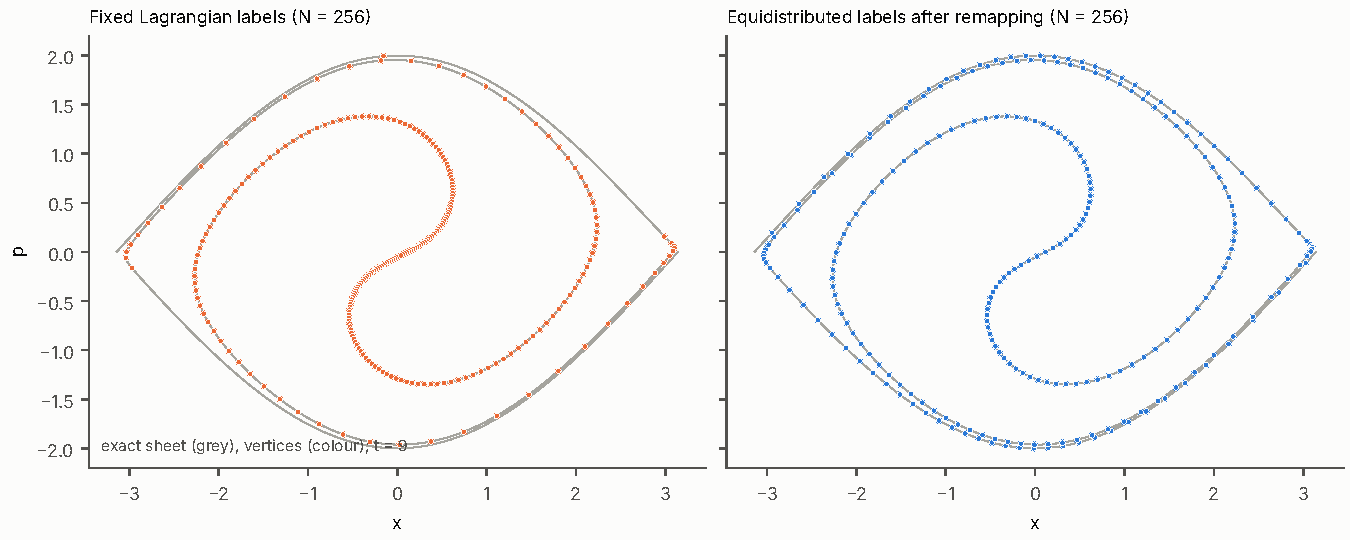
\includegraphics[width=0.86\textwidth]{../results/figures/fig_sheet.pdf}
\caption{Collapse test at $t=9$, $N=256$ vertices. Left: fixed Lagrangian labels leave the stretched outer
windings (labels near the stable manifold of the hyperbolic point) essentially unsampled. Right: labels after
optimal-transport remapping with the AC$(4,1)$ reconstruction. The label density varies by several orders of
magnitude; the mass per cell varies accordingly (\cref{prop:sampling}).}\label{fig:sheet}
\end{figure}

\begin{figure}[t]\centering
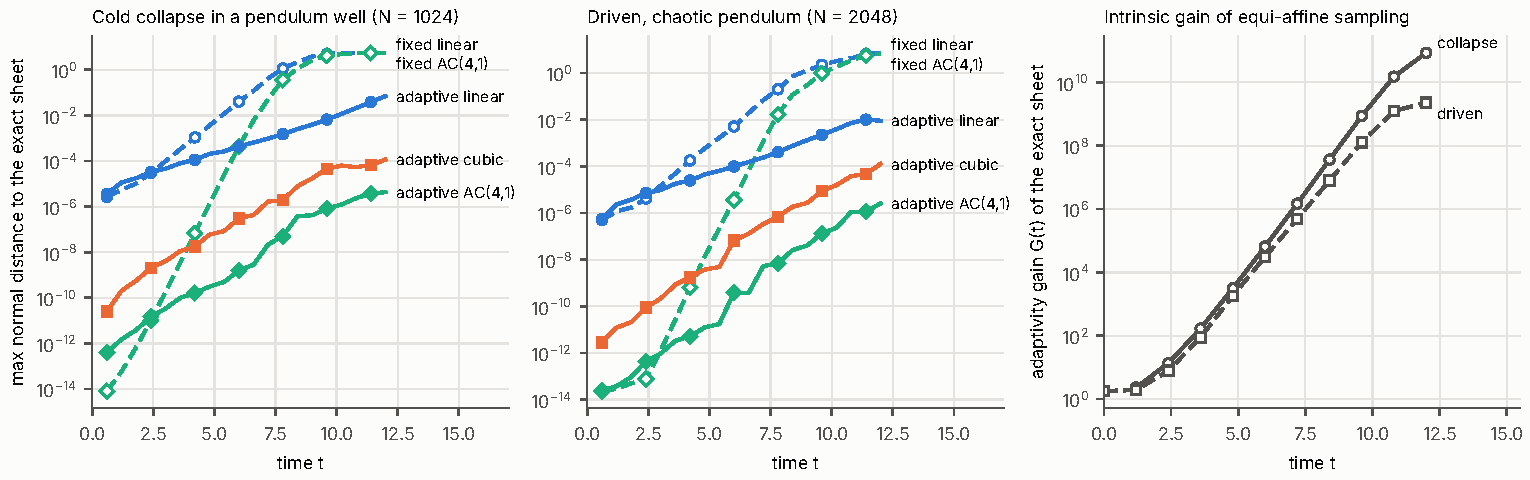
\includegraphics[width=\textwidth]{../results/figures/fig_history.pdf}
\caption{Normal error against the exact sheet for the collapse and driven tests (left, centre), and the
adaptivity gain $G(t)$ of \eqref{eq:complexity} for the exact sheets (right). Fixed sampling fails when $G$
becomes large, whatever the reconstruction; adaptive sampling with the action-corrected remap retains
$10^{-6}$.}\label{fig:history}
\end{figure}

\begin{table}[t]\centering\footnotesize
\resizebox{\textwidth}{!}{\TableHistory}
\caption{Final-time diagnostics, all tests ($c$: exact Liouville class; $E$: oracle energy). The total-mass error
is $0$ in every run (not shown). Remaps every 50, 20, 20, 25 steps respectively.}\label{tab:history}
\end{table}

\paragraph{Results.}
\emph{(1) Exact invariants.} For every action-corrected reconstruction the Poincar\'e invariant of the carrier
equals $c$ to round-off ($\le6\times10^{-15}$ absolute, with $c$ up to $16.3$) in all tests, for all $N$, and for
1 to 399 remaps (\cref{tab:history,tab:conv,tab:accum}), including the explicitly time-dependent Hamiltonians, as
\cref{thm:scheme}(ii) asserts. The interpolation remaps drift: linear by up to $-0.37$, cubic by up to
$3.8\times10^{-4}$, quintic by $6.7\times10^{-6}$ at 399 remaps, growing with the number of remaps as predicted by
\cref{thm:budget}; linear interpolation loses action monotonically (\cref{cex:polygon}).

\emph{(2) Accuracy.} On exact samples (fixed rows of \cref{tab:conv}) AC$(4,1)$ converges at order $5.00$ in the
normal direction against $4.00$ for the cubic it corrects, with tangential order 4 unchanged, confirming
\cref{thm:ac}(iii). With 39 remaps the adaptive AC$(4,1)$ run converges at order $\simeq4.6$ and is two to three
orders of magnitude more accurate than cubic remapping at equal $N$; AC$(6,1)$ reaches the round-off conditioning
floor of \cref{rem:roundoff} ($\sim10^{-9}$ at $N=4096$).

\emph{(3) Accumulation.} For AC$(4,1)$ the final normal error varies only between $1.7\times10^{-7}$ and
$9.4\times10^{-7}$ as the number of remaps goes from 1 to 399 (\cref{tab:accum}); the cubic remap degrades from
$2\times10^{-5}$ to $4.5\times10^{-4}$ and the linear one is destroyed. No instability is observed
(cf.\ \cref{obs:vn}).

\emph{(4) When adaptivity matters.} In the twist test the exact sheet has $G(t)\le21$: uniform labels are nearly
optimal and remapping buys nothing; with the same reconstruction the fixed mesh is more accurate than the
remapped one (\cref{tab:history}). This is an honest negative result for adaptivity on smooth phase mixing. In
the collapse and driven tests $G$ grows exponentially (\cref{tab:complexity}), reaching $10^{9}$--$10^{11}$ at
$t=12$, and the fixed mesh has normal error above $0.1$ from $t\approx7$--$8$ and $O(1)$ at the end for \emph{every} reconstruction, while the adaptive
action-corrected runs retain $e_\perp^{\max}=4\times10^{-6}$ ($N=1024$) and $3\times10^{-6}$ ($N=2048$). The smallest
label spacing produced by the remap at $t=12$ is $1.2\times10^{-6}$ against $6\times10^{-3}$ for uniform labels: a
fixed mesh would need several thousand times more vertices.

\emph{(5) Tangential error and mass.} The tangential error, which is the error in the \emph{placement of mass along
the sheet}, is not improved by the action (it is $O(h^m)$ for both families) and is the dominant error of the
action-corrected schemes ($3\times10^{-3}$ in the collapse test, concentrated where the sheet is exponentially
stretched and carries little mass; the mass-weighted $L^2$ normal error there is $10^{-7}$). Total mass is exact.

\emph{(6) A failure that taught something.} The first front implementation (parabolic arc as a graph over the
chord with a metric normal, tangential map by cubic interpolation; superseded and not retained in the repository) preserved the invariant exactly but converged
erratically; the maximal error sat at hairpin turns, where the phase-space speed $\abs{F'}$ is small and the
chord frame rotates by $O(1)$ between cells. The parametric form \eqref{eq:ac}, which commutes with affine symplectic
maps up to a higher-order term, removed the problem. We record it because it shows that \emph{exact invariants do
not imply accuracy}, and that equivariance under the affine symplectic group is a genuine design constraint.

\begin{figure}[t]\centering
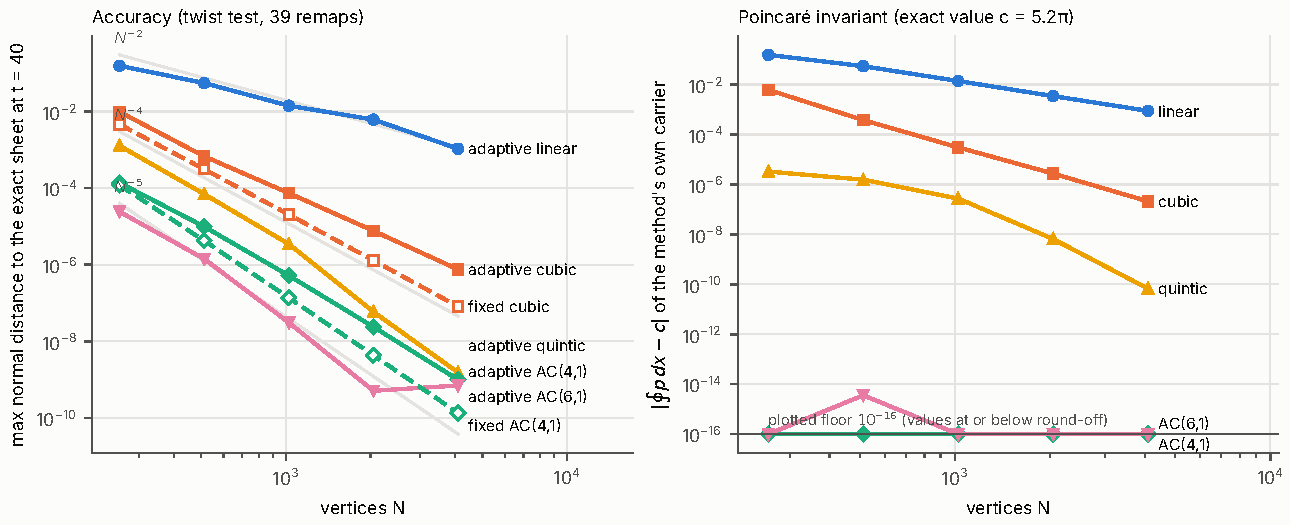
\includegraphics[width=0.92\textwidth]{../results/figures/fig_convergence.pdf}
\caption{Twist test, $t=40$, 39 remaps. Left: normal error versus $N$ (dashed: fixed Lagrangian mesh with the
same reconstruction). Right: error of the Poincar\'e invariant of each method's carrier; the action-corrected
schemes are at round-off (plotted at a floor).}\label{fig:conv}
\end{figure}

\begin{table}[t]\centering\footnotesize
\resizebox{\textwidth}{!}{\TableConvergence}
\caption{Twist test, $t=40$, 39 remaps (adaptive rows): $e_\perp^{\max}$ and observed order between the last two
resolutions (for AC$(6,1)$, between $N=1024$ and $2048$, the $N=4096$ value being at the conditioning floor).}\label{tab:conv}
\end{table}

\begin{figure}[t]\centering
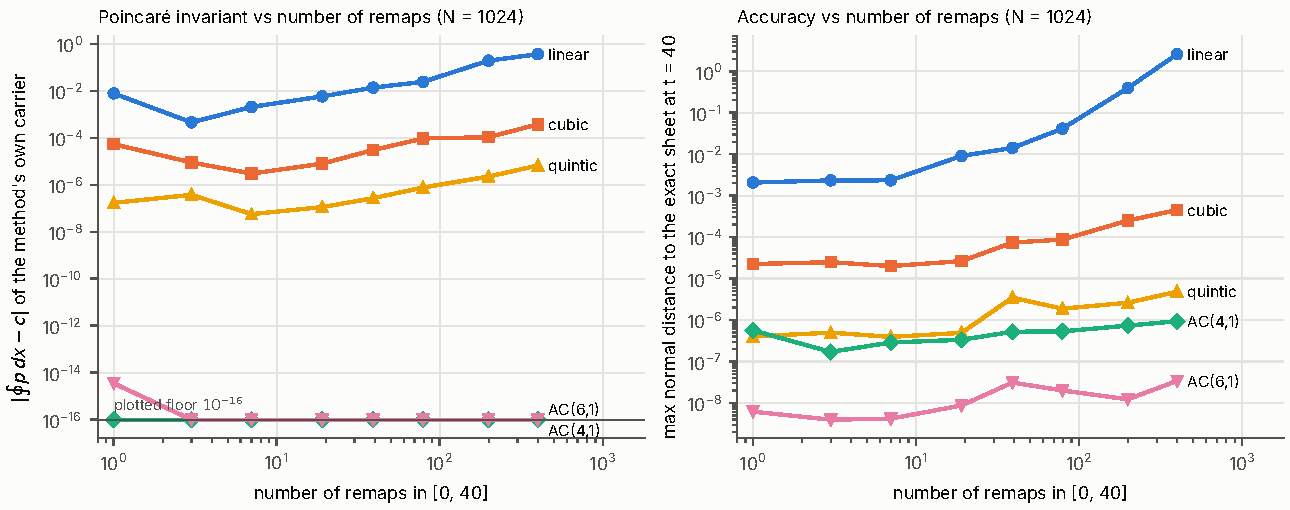
\includegraphics[width=0.92\textwidth]{../results/figures/fig_accumulation.pdf}
\caption{Twist test, $N=1024$: Poincar\'e invariant error and normal error at $t=40$ as functions of the number of
remaps.}\label{fig:accum}
\end{figure}

\begin{table}[t]\centering\scriptsize
\resizebox{\textwidth}{!}{\TableAccumulation}
\caption{Twist test, $N=1024$, $t=40$: dependence on the number of remaps.}\label{tab:accum}
\end{table}

\begin{table}[t]\centering\footnotesize
\TableComplexity
\caption{Intrinsic complexity of the exact sheets (oracle, $2^{16}$ labels): equi-affine length $\mathcal A$,
Euclidean length, maximal affine curvature and adaptivity gain $G$ of \eqref{eq:complexity}.}\label{tab:complexity}
\end{table}

\subsection{Four-dimensional phase space, single-stream regime}\label{sec:num2d}

\paragraph{Setup.} $\X=\T^2$, $H=\abs p^2/2+V(x)$,
$V=-(2\pi)^{-2}[\cos2\pi x_1+\cos2\pi x_2+\tfrac12\cos2\pi(x_1-x_2)]$, cold initial sheet $x=q$, $p=0$, $\Sigma=0$
($c=0$), $\Delta t=0.01$, $t\le0.9$ (linearised estimates: first shell crossing at $t\simeq1.11$, minimal $\det D_qx\simeq0.18$ at the end).
Reference grid $n\times n$, $n=32,64,128$. Remaps at steps 30, 50, 70: monitor
$M\propto(\norm C^2+(0.15\langle\norm C\rangle)^2)^{1/5}$ from the cubic form \eqref{eq:cubic}, mollified with a
Gaussian of label-space width $0.05$; Monge--Amp\`ere solve for $\varphi$; point location through the spectral
label map $\id+\nabla\varphi$. Reconstructions: bilinear, bicubic and biquintic splines of $(x,p)$ in $\xi$, and the
generating-function elements of \cref{thm:front} in the identity frame, \emph{front-3} ($x$: bicubic spline, $W$:
$C^1$ bicubic Hermite) and \emph{front-5} ($x$: biquintic spline, $W$: $C^2$ biquintic Hermite), with exact nodal
values and gradients \eqref{eq:hermitedata} and higher nodal derivatives from sixth-order differences of the gradient
data. Diagnostics: momentum error against the oracle at the nodes; circulation $\oint p_h\cdot\dd x_h$ of each
method's carrier along the images of 24 fixed circles in $\Xi$ (exact value $0$), by Richardson-extrapolated
trapezoid quadrature on 4096/8192 chords; total mass from the label cells.

\begin{figure}[t]\centering
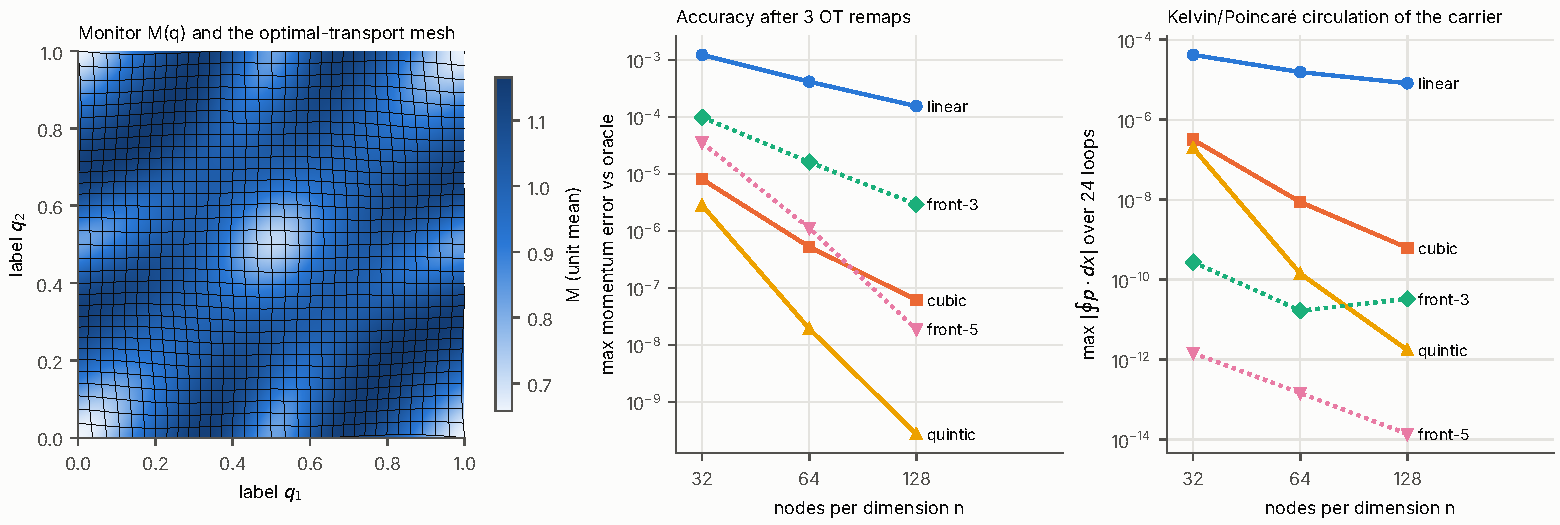
\includegraphics[width=\textwidth]{../results/figures/fig_2d.pdf}
\caption{$d=2$. Left: monitor on label space and the image of the reference grid under the optimal-transport map
($n=64$, every second line). Centre: momentum error after three remaps. Right: maximal circulation of each
carrier.}\label{fig:2d}
\end{figure}

\begin{table}[t]\centering\footnotesize
\resizebox{\textwidth}{!}{\TableTwoD}
\caption{$d=2$, $t=0.9$. Total-mass error $\le$\TwoDMassErr\ in all runs; cell masses vary by a factor up to
\TwoDMassRatio.}\label{tab:2d}
\end{table}

\begin{table}[t]\centering\footnotesize
\resizebox{\textwidth}{!}{\TableOT}
\caption{Monge--Amp\`ere solves of the front-5 run at $n=128$.}\label{tab:ot}
\end{table}

\paragraph{Results.}
\emph{Optimal transport.} The Newton--Krylov solver converges in 4--5 iterations to residual $10^{-13}$, with
$\lambda_{\min}(I+D^2\varphi)\ge0.86$ (\cref{tab:ot}); in a stand-alone test with monitor contrast $148$ it converged
in 6 iterations with $\lambda_{\min}=0.37$. The total mass computed from the label cells equals one to round-off
while individual cell masses vary (\cref{prop:mass,prop:sampling}).

\emph{Structure.} The carriers of the generating-function elements have circulation at the level of the loop
quadrature ($10^{-12}$--$10^{-14}$ for front-5; $10^{-11}$--$10^{-10}$ for front-3, whose momentum is only $C^0$ across cells,
which limits the extrapolated quadrature, not the identity $p_h\cdot\dd x_h=\dd W_h$). The spline carriers have a
genuine defect: $4\times10^{-5}\to8\times10^{-6}$ (bilinear), $3\times10^{-7}\to6\times10^{-10}$ (bicubic),
$2\times10^{-7}\to2\times10^{-12}$ (biquintic) for $n=32\to128$, larger than for the same reconstructions on exact
data (lower block of \cref{tab:2d}), i.e.\ created by the remaps.

\emph{Accuracy.} After three remaps the observed orders of the momentum error between successive resolutions are
$2.6,\,2.5$ for front-3 (third order on exact data) and $5.0,\,5.9$ for front-5, consistent with
\cref{thm:front}(iv); the plain splines of the same degree are about one order \emph{more} accurate in $p$
(bicubic: $3.9,\,3.1$; biquintic: $7.2,\,6.1$), because they interpolate $p$ directly whereas the front element
differentiates $W$. Thus in $d\ge2$, with the elements tested, exact Lagrangian structure costs one order of
momentum accuracy relative to an unconstrained spline of the same degree, in contrast to $d=1$ where the action
\emph{gains} one order. Since the monitor contrast is small here ($\le1.8$), adaptivity brings no accuracy gain in this
regime; the experiment demonstrates the mechanics and the structure, not a pay-off.

\emph{Monitor regularity.} With a non-smooth monitor ($\norm C$ with a mesh-scale smoother) and a bicubic label
map the remap errors of all higher-order reconstructions degraded to first order; \cref{rem:monreg} records the
remedy used above.

\paragraph{Limitations of the experimental evidence.} No self-consistent force; no multi-stream test in $d=2$
(the chart-wise element is singular at caustics, \cref{prob:glue}); no $d=3$ run; schedules rather than
error-controlled triggers; one family of monitors.

\section{Extension to comoving Vlasov--Poisson}\label{sec:cosmo}

\subsection{The comoving Hamiltonian and what carries over verbatim}

In comoving coordinates $x$ with canonical momentum $p=a^2\dot x$ (per unit mass) and cosmic time $t$,
\begin{equation}\label{eq:comoving}
H(x,p,t)=\frac{\abs p^2}{2a(t)^2}+\phi(x,t),\qquad\Delta_x\phi=\frac{3}{2}\,\Omega_mH_0^2\,\frac{\delta(x,t)}{a(t)},\qquad
\delta=\frac{\rho}{\bar\rho}-1,\quad\rho=(x_t)\pf\mu ,
\end{equation}
on the periodic box $\X=\T^3$ (zero mode of $\phi$ removed). The Hamiltonian is explicitly time dependent and, for
each $t$, separable. Everything in \cref{sec:continuum,sec:structure} was stated for time-dependent Hamiltonians:

\begin{proposition}[comoving sheets]\label{prop:comoving}\status{new derivation; corollary of \cref{thm:action,thm:carrier}}
For \eqref{eq:comoving} with $\phi_t\in C^2(\X)$ periodic: the sheet remains Lagrangian with constant Liouville class
(\cref{prop:invariants}); the kick--drift--kick scheme with $D_n=\int_{t_n}^{t_{n+1}}a^{-2}\dd t$ and kick factors
$\kappa=\int\dd t$ over the half steps \cite{QuinnEtAl1997} is a composition of exact symplectic maps of $T^*\X$ with
generating functions
\begin{equation}\label{eq:comovingaction}
A_{\rm drift}=\tfrac12D_n\abs p^2,\qquad A_{\rm kick}=-\kappa\,\phi_n(x),
\end{equation}
so the action is transported exactly and \cref{thm:carrier,thm:scheme} hold, with $\phi_n$ the potential actually
used for the force at the kick. Any other time variable (scale factor, superconformal time) only changes the
coefficients $D_n,\kappa$.
\end{proposition}

The comoving test of \cref{sec:num1d} is exactly this situation with a prescribed $\phi$: the Liouville class is
kept to within $5\times10^{-16}$ through $a\simeq11.7$ and 38 remaps, with $e_\perp^{\max}=2.8\times10^{-11}$ (\cref{tab:history}).
Energy is not conserved for \eqref{eq:comoving}; the Layzer--Irvine relation is a diagnostic, not an invariant, and
plays no role in the structure.

\subsection{Requirements imposed by the self-consistent coupling}

\begin{enumerate}[leftmargin=2em,itemsep=3pt]
\item \emph{Common-potential, exact-gradient force.} By \cref{rem:force} the force must be
$-\nabla\big(\sum_cW(x-x_c)\phi_c\big)$ with $W$ at least $C^1$, and the \emph{same} interpolated potential enters
$A_{\rm kick}$. Finite-difference-then-interpolate forces and forces derived variationally from the tessellated
potential energy both violate the hypothesis of \cref{thm:carrier}; with the former the pointwise relative curl of
the force is $O(h_{\rm grid})$.
\item \emph{Density deposit.} $\rho_h=(x_h)\pf(q_h^*\mu)$: each reference cell deposits its mass
$m_K=\mu(q_h(K))$ over the image $x_h(K)$ (exact polyhedral projection for P1 elements as in ColDICE; sub-sampling or
quadrature for curved carriers). Total deposited mass is exact by \cref{prop:mass} if the deposit is a partition of
unity. The deposit is \emph{not} required to be adjoint to the force interpolation; the price is that total
momentum and the $N$-vertex energy are conserved only to truncation order, the usual trade of energy-conserving
particle-mesh schemes \cite{HockneyEastwood}. Which of the two structures (one-particle symplecticity, needed for the
sheet; or exact momentum conservation) should be given up is a modelling decision; the sheet structure requires the former.
\item \emph{Initial data.} Zel'dovich data are exactly Lagrangian with the action \eqref{eq:zeldovich} and $c=0$;
second-order data are not (\cref{ex:ic}, \eqref{eq:2lpt}) and would freeze a third-order Lagrangian defect into the
carrier (\cref{thm:carrier}(ii)); they should be replaced by symplectically generated higher-order data.
\item \emph{Charts across caustics.} After shell crossing the identity frame fails on caustics. In $d=1$ the
edge-wise construction of \cref{thm:ac} handles any number of streams (all 1D tests above are multi-stream). In
$d=3$ a per-patch choice among the $2^3$ coordinate frames (or a rotation adapted to the patch) is needed, and
exactness across frame changes is \cref{prob:glue}.
\item \emph{Monitor.} The edge defects \eqref{eq:edgedefect} are available at no cost and are invariant under the
time-dependent canonical rescalings of \eqref{eq:comoving}. By \cref{rem:monreg} the monitor must be mollified at a
fixed comoving label scale.
\end{enumerate}

\subsection{What should be expected, and what should not}

\emph{Complexity.} The sheet volume and its affine complexity grow without bound inside collapsed structures;
in the externally driven chaotic test $\mathcal A$ grows by a factor $26$ and $G$ by $10^{9}$ over twelve dynamical
times (\cref{tab:complexity}). Optimal transport redistributes a fixed budget of vertices optimally with respect to
the monitor; it does not reduce $\mathcal A$. A production method needs $h$-refinement on top of the
$r$-adaptation (a finer reference mesh at a remap; \cref{thm:scheme} is indifferent to the number of nodes) and,
realistically, a fall-back to particles in regions of rapid mixing, as adopted by the sheet/release hybrid of
\cite{Stuecker2020}. Nothing in this note changes that assessment.

\emph{Regularity.} With singular caustic densities the tidal field is unbounded and the flow map is not $C^2$; the
error analysis of \cref{sec:error} then does not apply as stated, and the carrier's derivatives are controlled only
at the scale of the force-softening or mesh kernel. The structural statements (\cref{thm:carrier,thm:scheme}) are
unaffected, since they use only that each step is a $C^1$ symplectic map generated by a $C^2$ interpolated potential.

\emph{Stability of the coupling.} Whether exact preservation of the sheet invariants improves the long-time
fidelity of self-gravitating runs is an empirical question that the present prototype does not address.

\section{Proof ledger}\label{sec:ledger}

\begin{table}[h]\centering\footnotesize
\begin{tabular}{p{4.4cm}p{2.6cm}p{7.9cm}}\toprule
statement & status & basis / caveat\\\midrule
\cref{prop:vlasov,prop:invariants} sheet solves Vlasov; invariants & established & textbook (Cartan formula); self-consistent case under \cref{ass:regular}\\
\cref{thm:action} action transport, generating functions of kick/drift & established mathematics, new use & three-line proof; verified to round-off in all runs\\
\cref{ex:ic} Zel'dovich action; 2LPT defect \eqref{eq:2lpt} & new derivation & direct computation; consistent with known third-order transverse displacements\\
\cref{thm:gauge} relabelling invariance, ALE form & new derivation (elementary) & proved\\
\cref{thm:momentum} Lagrangian condition as momentum map & established \cite{Donaldson1999} & short verification given\\
\cref{prop:normalform} exact normal one-forms & new derivation (linear); nonlinear version \cite{Weinstein1971} & proved to first order\\
\cref{prop:cubic} cubic form & new derivation & proved; classical object\\
\cref{thm:ot,prop:ot1d} OT on the torus & established & cited; not re-proved\\
\cref{prop:sampling} sampling vs mass & new derivation (elementary) & proved\\
\cref{lem:edge,prop:flux} edge defect, P1 flux & new derivation & proved; symbolic check\\
\cref{prop:mass} mass as a degree & new derivation (elementary) & proved; $0$ / $10^{-16}$ in all runs\\
\cref{thm:carrier} carrier transport & new derivation & proved; requires common-potential force\\
\cref{thm:budget} invariant budget & new derivation & proved; drift with remap count observed\\
\cref{cex:polygon} polygon action loss & new derivation (elementary) & proved; numeric check\\
\cref{thm:rigidity} P1 rigidity on the lattice, $d=2$ & new derivation & proved (Fourier); kernel dimension $3n$ confirmed for $n=5,6,8$\\
\cref{obs:rigid} generic and $d=3$ rigidity & numerical observation & SVD ranks only; no proof\\
\cref{thm:ac} action-corrected interpolation & new derivation & (i),(ii),(iv) proved; (iii) proved to leading order, order confirmed for $m=4$ ($5.00$)\\
\cref{thm:front} generating-function elements & new derivation & proved (chart-wise); confirmed in $d=2$\\
\cref{thm:scheme} structure preservation of the scheme & new derivation & proved from the above\\
\cref{lem:lebesgue} Hermite constant 2 & new derivation (elementary) & proved\\
\cref{obs:vn} spectral radius $\le1$ & numerical observation & sampled grid; not a stability proof\\
\cref{thm:conv} convergence & new derivation, conditional & (R2) proved only for Lagrange and frozen-frame AC$(2,1)$\\
\cref{prop:comoving} comoving extension & corollary & proved for prescribed $\phi\in C^2$; external-potential test only\\
\cref{prob:glue} global Lagrangian carrier across caustics & open & no construction\\
uniform stability for unboundedly many remaps & open & evidence: \cref{obs:vn}, \cref{tab:accum}\\
self-consistent Vlasov--Poisson stability/convergence & open & not attempted\\
novelty of the action-based remap & unverified & limited literature check; ColDICE details beyond its abstract not re-verified\\\bottomrule
\end{tabular}
\caption{Ledger. ``New derivation'' means proved in this note; it is not a priority claim.}\label{tab:ledger}
\end{table}

\section{Verdict}\label{sec:verdict}

\paragraph{Feasibility.} Coupling Hamiltonian evolution to optimal-transport-guided remapping without
uncontrolled violation of invariants is \emph{feasible, with a precisely delimited scope}:
\begin{itemize}[leftmargin=1.6em,itemsep=2pt]
\item Mass: exact, in any dimension, by carrying labels (\cref{prop:mass}).
\item Hamiltonian structure between remaps: exact, in any dimension, given a common-potential exact-gradient
force (\cref{thm:carrier}); this is a constraint on force evaluation that existing particle-mesh practice does not
automatically meet.
\item Remaps, $d=1$: exact Liouville class and exact carrier for arbitrarily many remaps, any number of streams,
with a \emph{gain} of one order of accuracy (\cref{thm:ac}); demonstrated.
\item Remaps, $d\ge2$: exact chart-wise (\cref{thm:front}); demonstrated in $d=2$ before shell crossing, at the cost
of one order of momentum accuracy relative to unconstrained splines of equal degree. Across caustics exactness is
open (\cref{prob:glue}) and the fallback is the controlled budget of \cref{thm:budget}.
\end{itemize}

\paragraph{Fundamental obstructions.} (1) Exact preservation of $f$ is impossible for any projection. (2) Exact
element-wise Lagrangian structure is impossible for freely placed piecewise-linear elements
(\cref{thm:rigidity}); linear-order tessellations are Lagrangian only up to the cubic-form defect \eqref{eq:flux}.
(3) Conservative remapping and symplectic remapping constrain forms of different degree; neither implies the
other. (4) The structure-preserving perturbations of a sheet are exactly the graphs of exact one-forms
(\cref{prop:normalform}): one scalar degree of freedom out of $d$. The strongest viable alternative is therefore to
make the scalar the primary unknown, which is what the action-augmented representation does.

\paragraph{The role of optimal transport.} Modest and well defined: it is the canonical, tangle-free,
memoryless choice of the sampling map on label space. It contributes nothing to structure preservation (any
diffeomorphism would do), nothing in $d=1$ beyond equidistribution, and it cannot resolve anisotropy. Its
regularity requirement on the monitor is real and was observed.

\paragraph{Scientific novelty.} The combination of known algorithms is not the claim. What appears to be new, to
the limited extent we could check, is the structural analysis (carrier/budget, exact-normal-form
characterisation, P1 rigidity) and the remap that reconstructs the generating function from an exactly transported
action, with its invariant monitor. The closest antecedents are ColDICE's Poincar\'e-invariant refinement
criterion, Hermite (CIP-type) semi-Lagrangian interpolation, and traveltime interpolation in wavefront
construction; a proper literature review by specialists of geometric optics and of geometric integration is
required before any priority statement.

\paragraph{Recommended next steps.} (1) \Cref{prob:glue} in $d=2$: a two-frame construction across a fold caustic,
with a four-dimensional multi-stream test (the ColDICE two-sine-wave collapse is the natural benchmark). (2) A
proof of (R2) for AC$(m,1)$ and of power-boundedness. (3) Simplicial $C^1$ generating-function elements with
anisotropic $h$-refinement, to combine with ColDICE-type refinement. (4) A self-consistent 1D comoving test with an
exact-gradient particle-mesh force against the Zel'dovich solution, to quantify whether exact sheet invariants
matter in practice.


\begin{thebibliography}{99}\small
\bibitem{AbelHahnKaehler2012} T.~Abel, O.~Hahn, R.~Kaehler, Tracing the dark matter sheet in phase space, \emph{MNRAS} 427 (2012) 61.
\bibitem{ShandarinHabibHeitmann2012} S.~Shandarin, S.~Habib, K.~Heitmann, Cosmic web, multistream flows, and tessellations, \emph{Phys.\ Rev.\ D} 85 (2012) 083005.
\bibitem{HahnAbelKaehler2013} O.~Hahn, T.~Abel, R.~Kaehler, A new approach to simulating collisionless dark matter fluids, \emph{MNRAS} 434 (2013) 1171.
\bibitem{HahnAngulo2016} O.~Hahn, R.~E.~Angulo, An adaptively refined phase-space element method for cosmological simulations and collisionless dynamics, \emph{MNRAS} 455 (2016) 1115 (arXiv:1501.01959).
\bibitem{SousbieColombi2016} T.~Sousbie, S.~Colombi, ColDICE: a parallel Vlasov--Poisson solver using moving adaptive simplicial tessellation, \emph{J.\ Comput.\ Phys.} 321 (2016) 644 (arXiv:1509.07720).
\bibitem{ColombiTouma2014} S.~Colombi, J.~Touma, Vlasov--Poisson in 1D: waterbags, \emph{MNRAS} 441 (2014) 2414.
\bibitem{Stuecker2020} J.~St\"ucker, O.~Hahn, R.~E.~Angulo, S.~D.~M.~White, Simulating the complexity of the dark matter sheet I: numerical algorithms, \emph{MNRAS} 495 (2020) 4943.
\bibitem{VogelsbergerWhite2011} M.~Vogelsberger, S.~D.~M.~White, Streams and caustics: the fine-grained structure of $\Lambda$CDM haloes, \emph{MNRAS} 413 (2011) 1419.
\bibitem{ZhengMajda1994} Y.~Zheng, A.~Majda, Existence of global weak solutions to one-component Vlasov--Poisson and Fokker--Planck--Poisson systems in one space dimension with measures as initial data, \emph{Comm.\ Pure Appl.\ Math.} 47 (1994) 1365.
\bibitem{Arnold} V.~I.~Arnold, \emph{Mathematical Methods of Classical Mechanics}, 2nd ed., Springer, 1989.
\bibitem{Weinstein1971} A.~Weinstein, Symplectic manifolds and their Lagrangian submanifolds, \emph{Adv.\ Math.} 6 (1971) 329.
\bibitem{Donaldson1999} S.~K.~Donaldson, Moment maps and diffeomorphisms, \emph{Asian J.\ Math.} 3 (1999) 1.
\bibitem{Salmon1988} R.~Salmon, Hamiltonian fluid mechanics, \emph{Annu.\ Rev.\ Fluid Mech.} 20 (1988) 225.
\bibitem{FrischVillone2014} U.~Frisch, B.~Villone, Cauchy's almost forgotten Lagrangian formulation of the Euler equation for 3D incompressible flow, \emph{Eur.\ Phys.\ J.\ H} 39 (2014) 325.
\bibitem{ZheligovskyFrisch2014} V.~Zheligovsky, U.~Frisch, Time-analyticity of Lagrangian particle trajectories in ideal fluid flow, \emph{J.\ Fluid Mech.} 749 (2014) 404.
\bibitem{RampfVilloneFrisch2015} C.~Rampf, B.~Villone, U.~Frisch, How smooth are particle trajectories in a $\Lambda$CDM Universe?, \emph{MNRAS} 452 (2015) 1421.
\bibitem{Buchert1994} T.~Buchert, Lagrangian theory of gravitational instability of Friedman--Lema\^itre cosmologies: a generic third-order model for nonlinear clustering, \emph{MNRAS} 267 (1994) 811.
\bibitem{HLW} E.~Hairer, C.~Lubich, G.~Wanner, \emph{Geometric Numerical Integration}, 2nd ed., Springer, 2006.
\bibitem{MarsdenWest2001} J.~E.~Marsden, M.~West, Discrete mechanics and variational integrators, \emph{Acta Numer.} 10 (2001) 357.
\bibitem{QuinnEtAl1997} T.~Quinn, N.~Katz, J.~Stadel, G.~Lake, Time stepping N-body simulations, arXiv:astro-ph/9710043 (1997).
\bibitem{HockneyEastwood} R.~W.~Hockney, J.~W.~Eastwood, \emph{Computer Simulation Using Particles}, Adam Hilger, 1988.
\bibitem{Kraus2017} M.~Kraus, K.~Kormann, P.~J.~Morrison, E.~Sonnendr\"ucker, GEMPIC: geometric electromagnetic particle-in-cell methods, \emph{J.\ Plasma Phys.} 83 (2017) 905830401.
\bibitem{Brenier1991} Y.~Brenier, Polar factorization and monotone rearrangement of vector-valued functions, \emph{Comm.\ Pure Appl.\ Math.} 44 (1991) 375.
\bibitem{McCann2001} R.~J.~McCann, Polar factorization of maps on Riemannian manifolds, \emph{Geom.\ Funct.\ Anal.} 11 (2001) 589.
\bibitem{Cordero1999} D.~Cordero-Erausquin, Sur le transport de mesures p\'eriodiques, \emph{C.\ R.\ Acad.\ Sci.\ Paris S\'er.\ I} 329 (1999) 199.
\bibitem{Caffarelli1992} L.~A.~Caffarelli, The regularity of mappings with a convex potential, \emph{J.\ Amer.\ Math.\ Soc.} 5 (1992) 99.
\bibitem{Otto2001} F.~Otto, The geometry of dissipative evolution equations: the porous medium equation, \emph{Comm.\ Partial Differential Equations} 26 (2001) 101.
\bibitem{Villani2003} C.~Villani, \emph{Topics in Optimal Transportation}, AMS, 2003.
\bibitem{DelonSalomonSobolevski2010} J.~Delon, J.~Salomon, A.~Sobolevski, Fast transport optimization for Monge costs on the circle, \emph{SIAM J.\ Appl.\ Math.} 70 (2010) 2239.
\bibitem{BuddWilliams2006} C.~J.~Budd, J.~F.~Williams, Parabolic Monge--Amp\`ere methods for blow-up problems in several spatial dimensions, \emph{J.\ Phys.\ A} 39 (2006) 5425.
\bibitem{BuddHuangRussell2009} C.~J.~Budd, W.~Huang, R.~D.~Russell, Adaptivity with moving grids, \emph{Acta Numer.} 18 (2009) 111.
\bibitem{Delzanno2008} G.~L.~Delzanno, L.~Chac\'on, J.~M.~Finn, Y.~Chung, G.~Lapenta, An optimal robust equidistribution method for two-dimensional grid adaptation based on Monge--Kantorovich optimization, \emph{J.\ Comput.\ Phys.} 227 (2008) 9841.
\bibitem{Weller2016} H.~Weller, P.~Browne, C.~Budd, M.~Cullen, Mesh adaptation on the sphere using optimal transport and the numerical solution of a Monge--Amp\`ere type equation, \emph{J.\ Comput.\ Phys.} 308 (2016) 102.
\bibitem{HuangRussell2011} W.~Huang, R.~D.~Russell, \emph{Adaptive Moving Mesh Methods}, Springer, 2011.
\bibitem{FrischEtAl2002} U.~Frisch, S.~Matarrese, R.~Mohayaee, A.~Sobolevski, A reconstruction of the initial conditions of the Universe by optimal mass transportation, \emph{Nature} 417 (2002) 260.
\bibitem{BrenierEtAl2003} Y.~Brenier, U.~Frisch, M.~H\'enon, G.~Loeper, S.~Matarrese, R.~Mohayaee, A.~Sobolevski, Reconstruction of the early Universe as a convex optimization problem, \emph{MNRAS} 346 (2003) 501.
\bibitem{LevyEtAl2021} B.~L\'evy, R.~Mohayaee, S.~von~Hausegger, A fast semidiscrete optimal transport algorithm for a unique reconstruction of the early Universe, \emph{MNRAS} 506 (2021) 1165.
\bibitem{McClureVitale1975} D.~E.~McClure, R.~A.~Vitale, Polygonal approximation of plane convex bodies, \emph{J.\ Math.\ Anal.\ Appl.} 51 (1975) 326.
\bibitem{YabeAoki1991} T.~Yabe, T.~Aoki, A universal solver for hyperbolic equations by cubic-polynomial interpolation I. One-dimensional solver, \emph{Comput.\ Phys.\ Commun.} 66 (1991) 219.
\bibitem{VinjeEtAl1993} V.~Vinje, E.~Iversen, H.~Gj{\o}ystdal, Traveltime and amplitude estimation using wavefront construction, \emph{Geophysics} 58 (1993) 1157.
\bibitem{EngquistRunborg2003} B.~Engquist, O.~Runborg, Computational high frequency wave propagation, \emph{Acta Numer.} 12 (2003) 181.
\bibitem{Dritschel1988} D.~G.~Dritschel, Contour surgery: a topological reconnection scheme for extended integrations using contour dynamics, \emph{J.\ Comput.\ Phys.} 77 (1988) 240.
\bibitem{JRT2019} F.~Jauberteau, Y.~Rollin, S.~Tapie, Discrete geometry and isotropic surfaces, \emph{M\'em.\ Soc.\ Math.\ Fr.} 161 (2019) (arXiv:1802.08712).
\bibitem{WorseyFarin1987} A.~J.~Worsey, G.~Farin, An $n$-dimensional Clough--Tocher interpolant, \emph{Constr.\ Approx.} 3 (1987) 99.
\bibitem{BFS1965} F.~K.~Bogner, R.~L.~Fox, L.~A.~Schmit, The generation of interelement compatible stiffness and mass matrices by the use of interpolation formulas, \emph{Proc.\ Conf.\ Matrix Methods in Structural Mechanics}, Wright--Patterson AFB, 1965.
\bibitem{MyersColella2017} A.~Myers, P.~Colella, B.~Van~Straalen, A 4th-order particle-in-cell method with phase-space remapping for the Vlasov--Poisson equation, \emph{SIAM J.\ Sci.\ Comput.} 39 (2017) B467.
\end{thebibliography}

\end{document}
